\documentclass[12pt,a4paper]{report}
\usepackage[utf8]{vietnam}
\usepackage{amsmath}
\usepackage{amsfonts}
\usepackage{amssymb}
\usepackage{graphicx}
\usepackage[left=2cm,right=2cm,top=2cm,bottom=2cm]{geometry}

\usepackage{algorithm}
\usepackage{algorithmic}
\usepackage{mathtools}
\setcounter{secnumdepth}{4} % multi-level
\usepackage{subfig}
\usepackage{hyperref}

\usepackage{tabularx}
\begin{document}
\begin{table}[]

\caption{Ký Hiệu}
\label{my-label}
\renewcommand{\arraystretch}{2}
\hspace*{20mm}
\begin{tabular}{p{3cm} p{10cm} }
Ký hiệu & Ý nghĩa\\
\hline
a                                            & Một số thực                                          \\
\textbf{a}                                   & Một vector                                           \\
\textbf{A}                                   & Một ma trận                                          \\
$a_{i}$                                      & Phần tử thứ i của vector $\textbf{a}$                \\
$a_{ij}$                                     & Phần tử ở dòng i cột j của ma trận trận $\textbf{A}$ \\
$A_{i}$                                      & Dòng thứ i của ma trận $\textbf{A}$                  \\
$\textbf{A}^T$ & Ma trận chuyển vị của ma trận $\textbf{A}$           \\
$\mathbb{K}$                                 & Tập K                                                \\
$f(x)$                                       & Hàm số f với biến là x                               \\
$f'(x)$                              & Đạo hàm của hàm f(x)                                 \\
$\displaystyle f'_{x} $ hoặc $\displaystyle \frac{\partial f}{\partial x} $ & Đạo hàm riêng của  hàm f với x                       \\
$\nabla_\textbf{x}f$ & Gradient của hàm f theo vector \textbf{x}   \\

\end{tabular}
\end{table}

% ki hieu cho CNNs

\begin{table}[]

\caption{Ký Hiệu cho phần CNNs}
\label{my-label}
\renewcommand{\arraystretch}{2}
\hspace*{20mm}
\begin{tabular}{p{3cm} p{10cm} }
Ký hiệu & Ý nghĩa\\
\hline
$\textbf{x}^{(i)}$ 	& Dữ liệu thứ i của đầu vào (input)\\
$\textbf{X}$ 	& Ma trận dữ liệu đầu vào với $\textbf{x}^{(i)} $ là dòng thứ i trong ma trận $\textbf{X}_i$ \\

$\textbf{w}$ & Vector trọng số (weights) \\
$\textbf{W}$ & Ma trận trọng số\\

$l_i$ & Layer thứ i\\
$y_i$ & label của dữ liệu thứ i\\
$\widehat{\textbf{y}}$ & đầu ra ở lớp output (đầu ra dự đoán - predict)\\


\end{tabular}

\end{table}



\chapter{Nhắc lại kiến thức}

\everymath{\displaystyle}

\label{chap:chap2}
Trong chương này, tôi xin trình bày về các kiến thức cơ bản cần có để có thể thực hiện được bài toán đề ra.
\section{Ma trận}
\subsection{Định nghĩa}
Một ma trận \textbf{A} loại (cấp) $m_x n$ trên trường $\mathbb{K}$ ($\mathbb{K}$ – là trường thực $\mathbb{R}$ hoặc phức $\mathbb{C}$) là một bảng chữ nhật gồm $m x n$ phần tử trong $\mathbb{K}$ được viết thành $m$ dòng và $n$ cột như sau:
\begin{align*}
	\begin{bmatrix}
		a_1{}_1 & a_1{}_2 & a_1{}_3  &\ldots& a_1{}_n \\
		a_2{}_1 & a_2{}_2 & a_2{}_3  & \ldots & a_2{}_n \\
		a_3{}_1 & a_3{}_2 & a_3{}_3  & \ldots & a_3{}_n \\
		\vdots & \vdots& \vdots  & \ddots& \vdots\\			
		a_m{}_1 & a_m{}_2 & a_m{}_3 &\ldots& a_m{}_n \\
	\end{bmatrix}	
\end{align*}
Trong đó: \\ 

	\hspace{5mm} $a_{ij}$ là phần tử của ma trận A nằm ở giao điểm của dòng i và cột j\\
	
	\hspace{5mm} m : số dòng của ma trận \textbf{A}\\
	
	\hspace{5mm} n: số cột của ma trận \textbf{A}\\
	
	\hspace{5mm} 
$	\begin{bmatrix}
		a_{i1} & a_{i2}& a_{i3}&\ldots& a_{in}			
	\end{bmatrix}$ : 
	dòng thứ i của ma trận \textbf{A}\\
	
	\hspace{5mm}
	$\begin{bmatrix}	
		 a_{j1} \\ a_{j2}\\ a_{j3} \\ \vdots \\ a_{jm}		\end{bmatrix}$ : 
	  cột thứ j của ma trận \textbf{A}\\

\subsection{Phép cộng ma trận}
Cho hai ma trận \textbf{A}, \textbf{B} cùng cỡ  $ m_x n$, ta có tổng $\textbf{A} + \textbf{B}$ là ma trận có cùng kích thước ($m_x n$) với phần tử trong vị trí tương ứng bằng tổng của hai phần tử tương ứng của mỗi ma trận:
\begin{center}
$(\textbf{A}+\textbf{B}) = a_{ij}+b_{ij}$ với $ 1 \leq i \leq m$ và $1 \leq j \leq n$

\end{center}

Ví dụ:

$\begin{bmatrix}
   1 & 2 \\6 & 3
\end{bmatrix}$
+ 
$\begin{bmatrix}
3 & -2 \\
-4 & 1
\end{bmatrix}$
=
$\begin{bmatrix}
1+3 & 2 + -2 \\
6+-4 & 3+1
\end{bmatrix}$
=
$\begin{bmatrix}
4& 0\\
2 & 4
\end{bmatrix}$


\subsection{Phép nhân ma trận với ma trận}
Xét ma trận $\textbf{A}_m{}_x{}_p$ và ma trận \textbf{B}$_p{}_x{}_n$, trong đó số cột của ma trận \textbf{A} bằng số hàng của ma trận \textbf{B}.
Tích \textbf{A}\textbf{B} là ma trận \textbf{C} có m hàng và n cột, phần tử $c_i{}_j$ được xác định theo tích vô hướng của hàng tương ứng trong \textbf{A} với cột tương ứng trong \textbf{B}: 
\begin{align*}
c_i{}_j = a_i{}_1b_j{}_1 + a_i{}_2b_j{}_2 + \ldots + a_i{}_pb_j{}_p=
\sum_{k=1}^p(a_{ik}b_{jk})
\end{align*}

Ví dụ:\\

$\begin{bmatrix}
   1 & 2 \\6 & 3
\end{bmatrix}$
+ 
$\begin{bmatrix}
3 & -2 \\
-4 & 1
\end{bmatrix}$
=
$\begin{bmatrix}
1 * 3 + 2 * -4 & 1 * -2 + 2 * 1 \\
6 * 3 + 3 * -4  & 6 * -2 + 3 * 1
\end{bmatrix}$
=
$\begin{bmatrix}
-5 & 0\\
6 & -9
\end{bmatrix}$\\

Ngoài ra có một phép nhân khác được gọi là \textit{Hadamard} (hay \textit{element-wise}) được sử dụng khá nhiều trong học máy. Tích Hadamard của hai ma trận \textbf{cùng kích thước A, B} được kí hiệu là $\textbf{C}=\textbf{A} \odot \textbf{B}$, trong đó:
\begin{equation*}
c_{ij}=a_{ij}b_{ij}
\end{equation*}
\subsection{Ma trận chuyển vị}
Ma trận chuyển vị là một ma trận ở đó các hàng được thay thế bằng các cột, và ngược lại hay nói cách khác nếu ma trận \textbf{B} là ma trận chuyển vị của ma trận \textbf{A} thì: $b_{ij} = a_{ji}$ \par
Ma trận chuyển vị của ma trận $\textbf{A}$ được ký hiệu là $\textbf{A}^T$.\\ \par

$\begin{bmatrix}
a & b\\ c&d
\end{bmatrix}^T$
=
$\begin{bmatrix}
a&c\\b&d
\end{bmatrix}$
\section{Đạo hàm}
\subsection{Định nghĩa}
Cho hàm số ${ y=f(x)}$ xác định trên khoảng ${ (a;b)}$ (khoảng ${  (a;b)=\{x\in \mathbb {R} |a<x<b\}}$. Xét giá trị ${  x_{0}}$ và giá trị ${  x\in (a;b),x\neq x_{0}}$. \par 

Đặt $   \Delta x=x-x_0$ thì $  x = x_0+\Delta x$ và $\Delta x$ được gọi là số gia đối số. \par

Đặt $  \Delta y = f(x)-f(x_0)$ và $\Delta y$ được gọi là số gia hàm số. \par

Xét tỷ số ${  {\frac {\Delta y}{\Delta x}}}$. Nếu khi $  \Delta x\rightarrow0$, tỷ số đó dần tới một giới hạn thì giới hạn đó được gọi là đạo hàm của hàm số $  y=f(x)$ tại điểm $  x_0$ ký hiệu là ${  f'(x)}$\\

${  f'(x)=\lim _{\Delta x\rightarrow 0}{\frac {f(x_{0}+\Delta x)-f(x_{0})}{\Delta x}}}  $
\subsection{Đạo hàm riêng}
Đạo hàm riêng của một hàm số đa biến là đạo hàm theo một biến, các biến khác được xem như là hằng số. \par
Đạo hàm riêng của f đối với biến x được ký hiệu khác nhau bởi : ${  f'_x }$,  ${  \frac{\partial f}{\partial x} }.$\par
Ví dụ: Hàm số $f(x,y) = ax^2 + bxy + cy^5$ thì ta có:
\begin{itemize}
\setlength{\itemindent}{10mm}
	\item Đạo hàm theo x: ${  f'_x = 2ax +by}$
	\item Đạo hàm theo y: ${  f'_y = bx +5cy^4}$	
\end{itemize}

\textbf{Vector gradient}:
Cho một hàm số $f(\textbf{x})$ : $\mathbb{R}^n \rightarrow \mathbb{R}$. Trong trường hợp này f có các đạo hàm riêng $   \frac{\partial f}{\partial x_j}$ đối với mỗi biến $ x_j$ ($1\leq j \leq n$) thì vector chứa các đạo hàm riêng này là vector gradient.\par
\begin{center}

$ \nabla_\textbf{x}f(\textbf{x}) =
\renewcommand{\arraystretch}{2.5} 
\begin{bmatrix}

\frac{\partial f(\textbf{x})}{\partial x_1}\\ \frac{\partial f(\textbf{x})}{\partial x_2} \\ \vdots \\ \frac{\partial f(\textbf{x})}{\partial x_n}
\end{bmatrix}  $
\end{center}

\subsection{Đạo hàm hàm hợp (Chain rule)}

Đạo hàm hàm hợp là công thức để tính đạo hàm của hàm số gồm nhiều hàm số kết hợp với nhau. Đó là, nếu $f, g$ là hai hàm số và hàm $h(x) = f(g(x))$ thì ta có 
\begin{center}
$h'(x) = f(g(x))' = f'(g(x)).g'(x) $

\end{center}
hay chúng ta có công thức quen thuộc hơn với cách đặt $z=f(y), y=g(x)$:
\begin{center}
$\frac{dz}{dx} = \frac{dz}{dy} \frac{dy}{dz}$ = $f'(y)g'(x)$ = $f'(g(x)).g'(x)$
\end{center}

Ví dụ: Tính đạo hàm của hàm số $h=(x^2+5)^2$\par
 Đặt $g(x) = x^2 +5$ thì ta có $f(g) = g^2$, do đó $h'(x) = f'(g(x)).g'(x) = 2g2x= 4(x^2 +5)x$\par
%\textbf{Đạo hàm riêng của hàm hợp}: Giả sử ta có hàm số $f(u,v)$ trong đó $u(x,y)$ , $v(x,y)$ là các hàm số  theo biến $x,y$ và $f$ có đạo hàm riêng theo $u,v$ và $u,v$ có đạo hàm riêng theo $x,y$ thì ta có đạo hàm riêng của $f$ theo $x,y$ như sau:
%\begin{align*}
%	\begin{cases}
%        f'_{x} = f'_{u}u'_{x} +f'_{v}v'_{x}\\
%       f'_{y} = f'_{u}u'_{y} +f'_{v}v'_{y}
%    \end{cases}
%\end{align*}
%một cách biểu diễn khác
%\begin{align}
%	\begin{cases}
%		\frac{\partial f}{\partial x} = 
%		\frac{\partial f}{\partial u}\frac{\partial u}{\partial x} + 
%		\frac{\partial f}{\partial v}\frac{\partial v}{\partial x}\\[5mm]
%		\frac{\partial f}{\partial y} = \frac{\partial f}{\partial u}\frac{\partial u}{\partial y} +
%		 \frac{\partial f}{\partial v}\frac{\partial v}{\partial y}
%	\end{cases}
%\end{align}
\section{Ước lượng tham số bằng cực đại khả dĩ}
Ước lượng hợp lý cực đại (có người gọi là khả năng cực đại, tiếng Anh thường được viết là MLE, gọi tắt từ Maximum-Likelihood Estimation) là một kỹ thuật trong thống kê dùng để ước lượng giá trị tham số của một mô hình xác suất dựa trên những dữ liệu có được. Phương pháp này được đĩnh nghĩa như sau:\par
Giả sử $X=x_1,x_2,....,x_n$ là tập $n$ quan sát và $Y=y_1,y_2,...,y_n$ là số nhãn của quan sát; $x,y$ là hai biến độc lập ngẫu nhiên. Ta cần phải tìm tham số $\theta$ để biểu thức sau đây đạt được giá trị lớn nhất
\begin{equation}
\label{eq:ults}
h_{\theta} = P(Y|X;\theta)
\end{equation} 
hay biểu thức \ref{eq:ults} được viết lại như sau:
\begin{equation}
\widehat{\theta} = \arg\max_{\theta}P(Y|X;\theta)
\end{equation}
Do các quan sát là biến độc lập ngẫu nhiên nên ta có thể viết lại thành:
\begin{equation}
P(Y|X;\theta) = \prod^N_{i=1}P(y_i|x_i,\;\theta)
\end{equation}
Nhưng trực tiếp hàm số trên không hề đơn giản, hơn nữa khi N lớn thì tích của N số nhỏ hơn một có thể dẫn đến sai số trong tính toán. Một phương pháp thường được sử dụng đó là lấy logarit	tự nhiên (cơ số e) của hàm khả dĩ ta được:
\begin{equation}
l(P(Y|X;\theta)) = log\prod_{i=1}^N P(y_i|x_i;\theta)=\sum_{i=1}^NlogP(y_i|x_i;\theta)
\end{equation}
\section{Một vài phương pháp tối ưu}
Mục tiêu của bài toán tối ưu là tìm ra nghiệm \textit{global minimum}(điểm mà tại đó hàm số đạt giá trị nhỏ nhất) của hàm số.  Tuy nhiên, việc tìm global minimum của các hàm số là rất phức tạp, thậm chí là bất khả thi. Thay vào đó, người ta thường cố gắng tìm các điểm \textit{local minimum} (điểm cực tiểu), và ở một mức độ nào đó, coi đó là nghiệm cần tìm của bài toán.\par
Giả sử ta có $N$ quan sát $(\textbf{X},\textbf{y})$ có ánh xạ $\textbf{X} \to \textbf{Y}$ với $f(\mathbf{\theta},\textbf{X})=\textbf{y}$. Ta cần tìm global minimum cho hàm $f(\theta;\textbf{X},\textbf{y})$ trong đó $\mathbf{\theta}$ là một vector, $\theta=[\theta_1,\theta_2,...,\theta_m]$. Đạo hàm của hàm số đó tại một điểm   $\mathbf{\theta}$ bất kỳ được ký hiệu là $\nabla_\mathbf{\theta} f(\mathbf{\theta};\textbf{x},y)$
\subsection{Gradient descent}
Thuật toán gradient descent giúp ta tìm $\theta$ sao cho $f(\mathbf{\theta},\textbf{X})~\text{gần}~\textbf{y}$ nhất.
\begin{algorithm}[H]
\label{alg:grad}
\caption{Gradient desent}
\begin{algorithmic}[1]
\REQUIRE Tập $N$ quan sát (\textbf{X},\textbf{y})
\REQUIRE $\theta=[\theta_1,\theta_2,...,\theta_m]$
\REPEAT 
\FORALL {$i=1;i \leq N;i++$}
\STATE $\nabla \theta_i := - \nabla_{\theta}f(\theta;\textbf{x}_i,y_i)$
\ENDFOR
\STATE $\nabla \theta  =\frac{1}{N} \sum^{N}_{i=1}\nabla\theta_i$
\STATE Chọn bước nhảy $\eta$
\STATE Cập nhật $\theta := \theta - \eta\nabla\theta$

\UNTIL	thuật toán hội tụ
\end{algorithmic}
\end{algorithm}
Trong đó $\eta$ (đọc là eta) là một số dương được gọi là learning rate (tốc độ học) và giá trị của learning rate thường là 0.001. Việc lựa chọn learning rate rất quan trọng trong các bài toán thực tế. Việc lựa chọn giá trị này phụ thuộc nhiều vào từng bài toán và phải làm một vài thí nghiệm để chọn ra giá trị tốt nhất. Và dấu trừ tại $\nabla \theta := - \nabla_{\theta}f(\theta)$ thể hiện việc chúng ta phải đi\textit{ ngược với đạo hàm} (Đây cũng chính là lý do phương pháp này được gọi là Gradient Descent - descent nghĩa là đi ngược).\par
Nếu dữ liệu có kích thước $N$ lớn thì mỗi lần cập nhật $\theta$ đòi hỏi chúng ta sử dụng tất cả các quan sát $\textbf{x}_i$ do đó khối lượng tính toán lớn do phải tính đạo hàm trên toàn bộ dữ liệu, thuật toán chạy chậm. Do vậy để tiết kiệm khối lượng tính toán, chúng ta sẽ cập nhật tính toán sau mỗi dữ liệu quan sát, phương pháp này gọi là \textit{sochastic gradient descent (SGD)}

\begin{algorithm}[H]
\label{alg:sgd}
\caption{Stochastic Gradient descent}
\begin{algorithmic}[1]
\REQUIRE Tập $N$ quan sát (\textbf{X},\textbf{y})
\REQUIRE  $\theta=[\theta_1,\theta_2,...,\theta_m]$
\REPEAT 
\STATE Xáo trộn dữ liệu
\FORALL {$i=1;i \leq N;i++$}
\STATE $\nabla \theta_i := - \nabla_{\theta}f(\theta;\textbf{x}_i,y_i)$

\STATE Chọn bước nhảy $\eta$
\STATE Cập nhật $\theta := \theta + \eta\nabla\theta$
\IF {hội tụ}
	\STATE \text{break}
\ENDIF
\ENDFOR

\UNTIL	thuật toán hội tụ
\end{algorithmic}
\end{algorithm}
Khác với SGD, thay vì mỗi \textit{iteration} ta tính toán trên một quan sát thì ta sẽ tính toán với $k$ quan sát ($1<k\ll N$). Phương pháp này được gọi là \textit{mini-batch gradient descent.}

\begin{algorithm}[H]
\label{alg:minibatch}
\caption{Mini-batch Gradient descent}
\begin{algorithmic}[1]
\REQUIRE Tập n quan sát (\textbf{X},\textbf{y})
\REQUIRE $\theta=[\theta_1,\theta_2,...,\theta_m]$
\REPEAT 
\STATE Xáo trộn dữ liệu
\FORALL {$i=1;i \leq N;i=i+k$}
\STATE $\nabla \theta_i := -\sum^{i+k}_{j=i} \nabla_{\theta}f(\theta;\textbf{x}_j,y_j)$
\STATE Chọn bước nhảy $\eta$
\STATE Cập nhật $\theta := \theta - \eta\nabla\theta_i$
\IF {hội tụ}
	\STATE \text{break}
\ENDIF

\ENDFOR

\UNTIL	thuật toán hội tụ
\end{algorithmic} 

\end{algorithm}

\subsection{Gradient descents với Momentum}
Giả sử ta vẽ được một thung lũng như Hình \ref{fig:dothi}, ta thả một viên bi vào trong đó và mong muốn nó lăn đến điểm B, điểm sâu nhất của thung lũng. Nếu ta may mắn thả viên bi ở điểm A hoặc điểm G thì viên bi dễ dàng đến tiến điểm B. Nhưng nếu ta thả viên vi tại điểm D thì viên bi có thể sẽ giao động xung quanh điểm E và dừng tại đó do chưa đủ lực để đẩy viên bi qua điểm F rồi đến điểm G. Khi đó E chính là một điểm local minimum mà chúng ta không muốn. Do đó nếu ta tác động thêm một lực vào viên bi giúp nó có thể từ điểm E vượt qua F và tiến đến G. 
\begin{figure}[H]
\begin{center}
\label{fig:dothi}
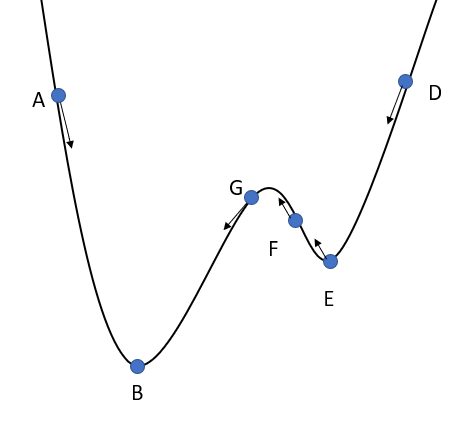
\includegraphics[scale=1]{chap2/image/momentum.png}
\caption{Đồ thị }
\end{center}
\end{figure}
Thuật toán gradient descent được ví như trọng lực tác dụng vào viên bi giúp nó di chuyển, B được coi điểm global minimum và E là một điểm local minimun. Để tránh hiện tượng nghiệm của gradient descent rơi vào một điểm local minimum không mong muốn thì ta tác động thêm một lực giúp gradient descent có thể bật ra khỏi vị trí của local minimum, lực này gọi là đà (\textit{momentum}). Vì thế cách cập nhật $\theta$ sẽ thay được thay đổi một chút như sau:
\begin{itemize}
\item[] $v_t:= \beta v_{t-1} +\eta \nabla\theta_{t}$
\item[]  $ \theta_t:= \theta_{t-1} - v_t$
\end{itemize}
Với $t$ là bước lặp thứ \textit{t}, biến $v$ được khởi tạo bằng 0 và trong tối ưu $\beta$ được gọi là đà (\textit{momentum}) với giá trị thường là $0.9$.
%\begin{algorithm}[H]
%\label{alg:momentum}
%\caption{Momentum kết hợp mini-batch}
%\begin{algorithmic}[1]
%\REQUIRE Tập n quan sát (\textbf{X},\textbf{y})
%\REQUIRE $\theta=[\theta_1,\theta_2,...,\theta_m]$
%\REPEAT 
%\STATE Xáo trộn dữ liệu
%\STATE v:=0
%\FORALL {$i=1;i \leq N;i=i+k$}
%\STATE $\nabla \theta_i := -\sum^{i+k}_{j=i} \nabla_{\theta}f(\theta;\textbf{x}_j,y_j)$
%\STATE $\mathit{v := mu*v+ \eta \nabla\theta_i}$
%\STATE Chọn bước nhảy $\eta$
%\STATE Cập nhật $\theta := \theta - v$
%\STATE if(hội tụ)
%\STATE break
%
%\ENDFOR
%
%\UNTIL	thuật toán hội tụ
%\end{algorithmic} 
%\end{algorithm}

\subsection{RMSprop}
\textit{RMSprop} là một cách giúp cho learning rate có thể thích nghi, điều chỉnh dựa trên độ lớn của gradient, được đưa ra bởi Geoff Hinton. Thuật toán này là một cách khắc phục việc dừng huấn luyện quá sớm khi áp dụng thuật toán Adagrad bằng cách chia learning rate cho . Khi áp dụng RMSprop, learning rate sẽ được thay đổi như sau:
\begin{itemize}
\item[] $m_t := \beta m_{t-1} + (1-\beta) \nabla\theta_{t}^2  $
\item[] $\theta_t := \theta_{t-1} - \frac{\eta}{\sqrt{m_{t-1}}+\epsilon}\nabla\theta_{t}$
\end{itemize}
Ta có biến $m$ được khởi tạo bằng 0 và $\beta$ là tốc độ giảm của learning rate, thường có giá trị là 0.9, 0.95 hoặc 0.99. Và $\epsilon$ giúp chúng ta tránh trường hợp chia cho 0, vì thế giá trị của $\epsilon$ thường là $10^{-8}$ 
\subsection{Adam}
\textit{Adam (Adaptive Moment Estimation)} là một bản cập nhật được đưa ra gần đây, nó khá giống với RMSprop và momentum. Cách cập nhật của thuật toán Adam như sau:
\begin{itemize}
\item[]  $m_t := \beta_1 m_{t-1} + (1-\beta_1) \nabla\theta_{t}$
\item[] $v_t := \beta_2 v_{t-1} + (1-\beta_2) \nabla\theta^2_{t}$
\item[] $ \widehat{m_t} := \frac{m_t}{1-\beta_1^{t}}$
\item[] $ \widehat{v_t} := \frac{v_t}{1-\beta_1^{t}} $
\item[] $\theta_t := \theta_1 + \frac{\eta }{\sqrt{\widehat{v_t}} +\epsilon}\widehat{m_t}$ 
\end{itemize}
$m_t,~v_t$ là giá trị ước lượng giữa thời điểm trước và thời điểm sau của các gradient tương ứng. Các giá trị của $m_t,~v_t$ đều được khởi tạo bằng 0. Các tác giả của Adam thấy rằng chúng bị lệch về 0, đặc biệt là các bước lặp đầu. Do vậy họ tạo ra $\widehat{m_t}~\text{và}~\widehat{v_t}$ để chống lại việc giá trị của $m_t ~\text{và}~ v_t$ lệch về 0. Các giá trị của $\beta_1,~\beta_2$ được tác giả đề xuất là 0.9 cho $\beta_1$, 0.999 cho $\beta2$  và $10^{-8} ~\text{cho}~ \epsilon$ như ở RMSprop.


\everymath{\displaystyle}  

\chapter{Cơ Sở Lý Thuyết}
\label{chap:chap3}
\section{Kiến thức toán và xắc suất}
\hspace{5mm} Trong phần này, tôi xin trình bày về các kiến thức cơ bản về toán và xắc suất cần có để có thể thực hiện được bài toán đề ra.
\subsection{Ma trận}
\subsubsection{Định nghĩa}
\hspace{5mm} Một ma trận \textbf{A} loại (cấp) $m_x n$ trên trường $\mathbb{K}$ ($\mathbb{K}$ – là trường thực $\mathbb{R}$ hoặc phức $\mathbb{C}$) là một bảng chữ nhật gồm $m x n$ phần tử trong $\mathbb{K}$ được viết thành $m$ dòng và $n$ cột như sau:
\begin{align*}
	\begin{bmatrix}
		a_1{}_1 & a_1{}_2 & a_1{}_3  &\ldots& a_1{}_n \\
		a_2{}_1 & a_2{}_2 & a_2{}_3  & \ldots & a_2{}_n \\
		a_3{}_1 & a_3{}_2 & a_3{}_3  & \ldots & a_3{}_n \\
		\vdots & \vdots& \vdots  & \ddots& \vdots\\			
		a_m{}_1 & a_m{}_2 & a_m{}_3 &\ldots& a_m{}_n \\
	\end{bmatrix}	
\end{align*}
Trong đó: \\ 

	\hspace{5mm} $a_{ij}$ là phần tử của ma trận A nằm ở giao điểm của dòng i và cột j\\
	
	\hspace{5mm} m : số dòng của ma trận \textbf{A}\\
	
	\hspace{5mm} n: số cột của ma trận \textbf{A}\\
	
	\hspace{5mm} 
$	\begin{bmatrix}
		a_{i1} & a_{i2}& a_{i3}&\ldots& a_{in}			
	\end{bmatrix}$ : 
	dòng thứ i của ma trận \textbf{A}\\
	
	\hspace{5mm}
	$\begin{bmatrix}	
		 a_{j1} \\ a_{j2}\\ a_{j3} \\ \vdots \\ a_{jm}		\end{bmatrix}$ : 
	  cột thứ j của ma trận \textbf{A}\\

\subsubsection{Phép cộng ma trận}
\hspace{5mm} Cho hai ma trận \textbf{A}, \textbf{B} cùng cỡ  $ m_x n$, ta có tổng $\textbf{A} + \textbf{B}$ là ma trận có cùng kích thước ($m_x n$) với phần tử trong vị trí tương ứng bằng tổng của hai phần tử tương ứng của mỗi ma trận:
\begin{center}
$(\textbf{A}+\textbf{B}) = a_{ij}+b_{ij}$ với $ 1 \leq i \leq m$ và $1 \leq j \leq n$

\end{center}

Ví dụ:

$\begin{bmatrix}
   1 & 2 \\6 & 3
\end{bmatrix}$
+ 
$\begin{bmatrix}
3 & -2 \\
-4 & 1
\end{bmatrix}$
=
$\begin{bmatrix}
1+3 & 2 + -2 \\
6+-4 & 3+1
\end{bmatrix}$
=
$\begin{bmatrix}
4& 0\\
2 & 4
\end{bmatrix}$


\subsubsection{Phép nhân ma trận với ma trận}
Xét ma trận $\textbf{A}_m{}_x{}_p$ và ma trận \textbf{B}$_p{}_x{}_n$, trong đó số cột của ma trận \textbf{A} bằng số hàng của ma trận \textbf{B}.
\hspace{5mm} Tích \textbf{A}\textbf{B} là ma trận \textbf{C} có m hàng và n cột, phần tử $c_i{}_j$ được xác định theo tích vô hướng của hàng tương ứng trong \textbf{A} với cột tương ứng trong \textbf{B}: 
\begin{align*}
c_i{}_j = a_i{}_1b_j{}_1 + a_i{}_2b_j{}_2 + \ldots + a_i{}_pb_j{}_p=
\sum_{k=1}^p(a_{ik}b_{jk})
\end{align*}

Ví dụ:\\

$\begin{bmatrix}
   1 & 2 \\6 & 3
\end{bmatrix}$
+ 
$\begin{bmatrix}
3 & -2 \\
-4 & 1
\end{bmatrix}$
=
$\begin{bmatrix}
1 * 3 + 2 * -4 & 1 * -2 + 2 * 1 \\
6 * 3 + 3 * -4  & 6 * -2 + 3 * 1
\end{bmatrix}$
=
$\begin{bmatrix}
-5 & 0\\
6 & -9
\end{bmatrix}$\\

Ngoài ra có một phép nhân khác được gọi là \textit{Hadamard} (hay \textit{element-wise}) được sử dụng khá nhiều trong học máy. Tích Hadamard của hai ma trận \textbf{cùng kích thước A, B} được kí hiệu là $\textbf{C}=\textbf{A} \odot \textbf{B}$, trong đó:
\begin{equation*}
c_{ij}=a_{ij}b_{ij}
\end{equation*}
\subsubsection{Ma trận chuyển vị}
\hspace{5mm} Ma trận chuyển vị là một ma trận ở đó các hàng được thay thế bằng các cột, và ngược lại hay nói cách khác nếu ma trận \textbf{B} là ma trận chuyển vị của ma trận \textbf{A} thì: $b_{ij} = a_{ji}$ \par
Ma trận chuyển vị của ma trận $\textbf{A}$ được ký hiệu là $\textbf{A}^T$.\\ \par

$\begin{bmatrix}
a & b\\ c&d
\end{bmatrix}^T$
=
$\begin{bmatrix}
a&c\\b&d
\end{bmatrix}$
\subsection{Đạo hàm}
\subsubsection{Định nghĩa}
\hspace{5mm} Cho hàm số ${ y=f(x)}$ xác định trên khoảng ${ (a;b)}$ (khoảng ${  (a;b)=\{x\in \mathbb {R} |a<x<b\}}$. Xét giá trị ${  x_{0}}$ và giá trị ${  x\in (a;b),x\neq x_{0}}$. \par 

Đặt $   \Delta x=x-x_0$ thì $  x = x_0+\Delta x$ và $\Delta x$ được gọi là số gia đối số. \par

Đặt $  \Delta y = f(x)-f(x_0)$ và $\Delta y$ được gọi là số gia hàm số. \par

Xét tỷ số ${  {\frac {\Delta y}{\Delta x}}}$. Nếu khi $  \Delta x\rightarrow0$, tỷ số đó dần tới một giới hạn thì giới hạn đó được gọi là đạo hàm của hàm số $  y=f(x)$ tại điểm $  x_0$ ký hiệu là ${  f'(x)}$\\

${  f'(x)=\lim _{\Delta x\rightarrow 0}{\frac {f(x_{0}+\Delta x)-f(x_{0})}{\Delta x}}}  $
\subsubsection{Đạo hàm riêng}
Đạo hàm riêng của một hàm số đa biến là đạo hàm theo một biến, các biến khác được xem như là hằng số. \par
Đạo hàm riêng của f đối với biến x được ký hiệu khác nhau bởi : ${  f'_x }$,  ${  \frac{\partial f}{\partial x} }.$\par
Ví dụ: Hàm số $f(x,y) = ax^2 + bxy + cy^5$ thì ta có:
\begin{itemize}
\setlength{\itemindent}{10mm}
	\item Đạo hàm theo x: ${  f'_x = 2ax +by}$
	\item Đạo hàm theo y: ${  f'_y = bx +5cy^4}$	
\end{itemize}

\textbf{Vector gradient}:
Cho một hàm số $f(\textbf{x})$ : $\mathbb{R}^n \rightarrow \mathbb{R}$. Trong trường hợp này f có các đạo hàm riêng $   \frac{\partial f}{\partial x_j}$ đối với mỗi biến $ x_j$ ($1\leq j \leq n$) thì vector chứa các đạo hàm riêng này là vector gradient.\par
\begin{center}

$ \nabla_\textbf{x}f(\textbf{x}) =
\renewcommand{\arraystretch}{2.5} 
\begin{bmatrix}

\frac{\partial f(\textbf{x})}{\partial x_1}\\ \frac{\partial f(\textbf{x})}{\partial x_2} \\ \vdots \\ \frac{\partial f(\textbf{x})}{\partial x_n}
\end{bmatrix}  $
\end{center}

\subsubsection{Đạo hàm hàm hợp (Chain rule)}

\hspace{5mm} Đạo hàm hàm hợp là công thức để tính đạo hàm của hàm số gồm nhiều hàm số kết hợp với nhau. Đó là, nếu $f, g$ là hai hàm số và hàm $h(x) = f(g(x))$ thì ta có 
\begin{center}
$h'(x) = f(g(x))' = f'(g(x)).g'(x) $

\end{center}
hay chúng ta có công thức quen thuộc hơn với cách đặt $z=f(y), y=g(x)$:
\begin{center}
$\frac{dz}{dx} = \frac{dz}{dy} \frac{dy}{dz}$ = $f'(y)g'(x)$ = $f'(g(x)).g'(x)$
\end{center}

Ví dụ: Tính đạo hàm của hàm số $h=(x^2+5)^2$\par
 Đặt $g(x) = x^2 +5$ thì ta có $f(g) = g^2$, do đó $h'(x) = f'(g(x)).g'(x) = 2g2x= 4(x^2 +5)x$\par
%\textbf{Đạo hàm riêng của hàm hợp}: Giả sử ta có hàm số $f(u,v)$ trong đó $u(x,y)$ , $v(x,y)$ là các hàm số  theo biến $x,y$ và $f$ có đạo hàm riêng theo $u,v$ và $u,v$ có đạo hàm riêng theo $x,y$ thì ta có đạo hàm riêng của $f$ theo $x,y$ như sau:
%\begin{align*}
%	\begin{cases}
%        f'_{x} = f'_{u}u'_{x} +f'_{v}v'_{x}\\
%       f'_{y} = f'_{u}u'_{y} +f'_{v}v'_{y}
%    \end{cases}
%\end{align*}
%một cách biểu diễn khác
%\begin{align}
%	\begin{cases}
%		\frac{\partial f}{\partial x} = 
%		\frac{\partial f}{\partial u}\frac{\partial u}{\partial x} + 
%		\frac{\partial f}{\partial v}\frac{\partial v}{\partial x}\\[5mm]
%		\frac{\partial f}{\partial y} = \frac{\partial f}{\partial u}\frac{\partial u}{\partial y} +
%		 \frac{\partial f}{\partial v}\frac{\partial v}{\partial y}
%	\end{cases}
%\end{align}
\subsection{Ước lượng tham số bằng cực đại khả dĩ}
\hspace{5mm} Ước lượng hợp lý cực đại (có người gọi là khả năng cực đại, tiếng Anh thường được viết là MLE, gọi tắt từ Maximum-Likelihood Estimation) là một kỹ thuật trong thống kê dùng để ước lượng giá trị tham số của một mô hình xác suất dựa trên những dữ liệu có được. Phương pháp này được đĩnh nghĩa như sau:\par
Giả sử $X=x_1,x_2,....,x_n$ là tập $n$ quan sát và $Y=y_1,y_2,...,y_n$ là số nhãn của quan sát; $x,y$ là hai biến độc lập ngẫu nhiên. Ta cần phải tìm tham số $\theta$ để biểu thức sau đây đạt được giá trị lớn nhất
\begin{equation}
\label{eq:ults}
h_{\theta} = P(Y|X;\theta)
\end{equation} 
hay biểu thức \ref{eq:ults} được viết lại như sau:
\begin{equation}
\widehat{\theta} = \arg\max_{\theta}P(Y|X;\theta)
\end{equation}
Do các quan sát là biến độc lập ngẫu nhiên nên ta có thể viết lại thành:
\begin{equation}
P(Y|X;\theta) = \prod^N_{i=1}P(y_i|x_i,\;\theta)
\end{equation}
Nhưng trực tiếp hàm số trên không hề đơn giản, hơn nữa khi N lớn thì tích của N số nhỏ hơn một có thể dẫn đến sai số trong tính toán. Một phương pháp thường được sử dụng đó là lấy logarit	tự nhiên (cơ số e) của hàm khả dĩ ta được:
\begin{equation}
l(P(Y|X;\theta)) = log\prod_{i=1}^N P(y_i|x_i;\theta)=\sum_{i=1}^NlogP(y_i|x_i;\theta)
\end{equation}
\subsection{Một vài phương pháp tối ưu}
\label{sec:toiuu}
\hspace{5mm} Mục tiêu của bài toán tối ưu là tìm ra nghiệm \textit{global minimum}(điểm mà tại đó hàm số đạt giá trị nhỏ nhất) của hàm số.  Tuy nhiên, việc tìm global minimum của các hàm số là rất phức tạp, thậm chí là bất khả thi. Thay vào đó, người ta thường cố gắng tìm các điểm \textit{local minimum} (điểm cực tiểu), và ở một mức độ nào đó, coi đó là nghiệm cần tìm của bài toán.\par
Giả sử ta có $N$ quan sát $(\textbf{X},\textbf{y})$ có ánh xạ $\textbf{X} \to \textbf{Y}$ với $f(\mathbf{\theta},\textbf{X})=\textbf{y}$. Ta cần tìm global minimum cho hàm $f(\theta;\textbf{X},\textbf{y})$ trong đó $\mathbf{\theta}$ là một vector, $\theta=[\theta_1,\theta_2,...,\theta_m]$. Đạo hàm của hàm số đó tại một điểm   $\mathbf{\theta}$ bất kỳ được ký hiệu là $\nabla_\mathbf{\theta} f(\mathbf{\theta};\textbf{x},y)$
\subsubsection{Gradient descent}
\hspace{5mm} Thuật toán gradient descent giúp ta tìm $\theta$ sao cho $f(\mathbf{\theta},\textbf{X})~\text{gần}~\textbf{y}$ nhất.
\begin{algorithm}[H]
\label{alg:grad}
\caption{Gradient desent}
\begin{algorithmic}[1]
\REQUIRE Tập $N$ quan sát (\textbf{X},\textbf{y})
\REQUIRE $\theta=[\theta_1,\theta_2,...,\theta_m]$
\REPEAT 
\FORALL {$i=1;i \leq N;i++$}
\STATE $\nabla \theta_i := - \nabla_{\theta}f(\theta;\textbf{x}_i,y_i)$
\ENDFOR
\STATE $\nabla \theta  =\frac{1}{N} \sum^{N}_{i=1}\nabla\theta_i$
\STATE Chọn bước nhảy $\eta$
\STATE Cập nhật $\theta := \theta - \eta\nabla\theta$

\UNTIL	thuật toán hội tụ
\end{algorithmic}
\end{algorithm}
Trong đó $\eta$ (đọc là eta) là một số dương được gọi là learning rate (tốc độ học) và giá trị của learning rate thường là 0.001. Việc lựa chọn learning rate rất quan trọng trong các bài toán thực tế. Việc lựa chọn giá trị này phụ thuộc nhiều vào từng bài toán và phải làm một vài thí nghiệm để chọn ra giá trị tốt nhất. Và dấu trừ tại $\nabla \theta := - \nabla_{\theta}f(\theta)$ thể hiện việc chúng ta phải đi\textit{ ngược với đạo hàm} (Đây cũng chính là lý do phương pháp này được gọi là Gradient Descent - descent nghĩa là đi ngược).\par
Nếu dữ liệu có kích thước $N$ lớn thì mỗi lần cập nhật $\theta$ đòi hỏi chúng ta sử dụng tất cả các quan sát $\textbf{x}_i$ do đó khối lượng tính toán lớn do phải tính đạo hàm trên toàn bộ dữ liệu, thuật toán chạy chậm. Do vậy để tiết kiệm khối lượng tính toán, chúng ta sẽ cập nhật tính toán sau mỗi dữ liệu quan sát, phương pháp này gọi là \textit{sochastic gradient descent (SGD)}

\begin{algorithm}[H]
\label{alg:sgd}
\caption{Stochastic Gradient descent}
\begin{algorithmic}[1]
\REQUIRE Tập $N$ quan sát (\textbf{X},\textbf{y})
\REQUIRE  $\theta=[\theta_1,\theta_2,...,\theta_m]$
\REPEAT 
\STATE Xáo trộn dữ liệu
\FORALL {$i=1;i \leq N;i++$}
\STATE $\nabla \theta_i := - \nabla_{\theta}f(\theta;\textbf{x}_i,y_i)$

\STATE Chọn bước nhảy $\eta$
\STATE Cập nhật $\theta := \theta + \eta\nabla\theta$
\IF {hội tụ}
	\STATE \text{break}
\ENDIF
\ENDFOR

\UNTIL	thuật toán hội tụ
\end{algorithmic}
\end{algorithm}
Khác với SGD, thay vì mỗi \textit{iteration} ta tính toán trên một quan sát thì ta sẽ tính toán với $k$ quan sát ($1<k\ll N$). Phương pháp này được gọi là \textit{mini-batch gradient descent.}

\begin{algorithm}[H]
\label{alg:minibatch}
\caption{Mini-batch Gradient descent}
\begin{algorithmic}[1]
\REQUIRE Tập n quan sát (\textbf{X},\textbf{y})
\REQUIRE $\theta=[\theta_1,\theta_2,...,\theta_m]$
\REPEAT 
\STATE Xáo trộn dữ liệu
\FORALL {$i=1;i \leq N;i=i+k$}
\STATE $\nabla \theta_i := -\sum^{i+k}_{j=i} \nabla_{\theta}f(\theta;\textbf{x}_j,y_j)$
\STATE Chọn bước nhảy $\eta$
\STATE Cập nhật $\theta := \theta - \eta\nabla\theta_i$
\IF {hội tụ}
	\STATE \text{break}
\ENDIF

\ENDFOR

\UNTIL	thuật toán hội tụ
\end{algorithmic} 

\end{algorithm}

\subsubsection{Gradient descents với Momentum}
\hspace{5mm}  Giả sử ta vẽ được một thung lũng như Hình \ref{fig:dothi}, ta thả một viên bi vào trong đó và mong muốn nó lăn đến điểm B, điểm sâu nhất của thung lũng. Nếu ta may mắn thả viên bi ở điểm A hoặc điểm G thì viên bi dễ dàng đến tiến điểm B. Nhưng nếu ta thả viên vi tại điểm D thì viên bi có thể sẽ giao động xung quanh điểm E và dừng tại đó do chưa đủ lực để đẩy viên bi qua điểm F rồi đến điểm G. Khi đó E chính là một điểm local minimum mà chúng ta không muốn. Do đó nếu ta tác động thêm một lực vào viên bi giúp nó có thể từ điểm E vượt qua F và tiến đến G. 
\begin{figure}[H]
\begin{center}
\label{fig:dothi}
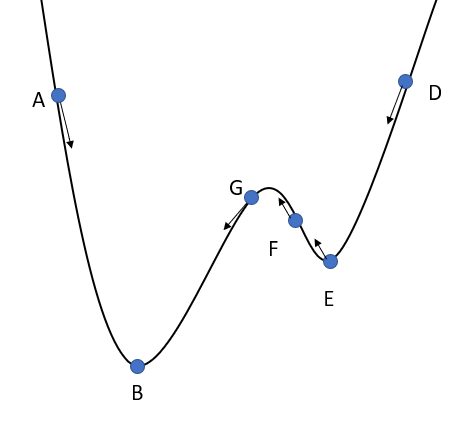
\includegraphics[scale=1]{chap2/image/momentum.png}
\caption{Đồ thị }
\end{center}
\end{figure}
Thuật toán gradient descent được ví như trọng lực tác dụng vào viên bi giúp nó di chuyển, B được coi điểm global minimum và E là một điểm local minimun. Để tránh hiện tượng nghiệm của gradient descent rơi vào một điểm local minimum không mong muốn thì ta tác động thêm một lực giúp gradient descent có thể bật ra khỏi vị trí của local minimum, lực này gọi là đà (\textit{momentum}). Vì thế cách cập nhật $\theta$ sẽ thay được thay đổi một chút như sau:
\begin{itemize}
\item[] $v_t:= \beta v_{t-1} +\eta \nabla\theta_{t}$
\item[]  $ \theta_t:= \theta_{t-1} - v_t$
\end{itemize}
Với $t$ là bước lặp thứ \textit{t}, biến $v$ được khởi tạo bằng 0 và trong tối ưu $\beta$ được gọi là đà (\textit{momentum}) với giá trị thường là $0.9$.
%\begin{algorithm}[H]
%\label{alg:momentum}
%\caption{Momentum kết hợp mini-batch}
%\begin{algorithmic}[1]
%\REQUIRE Tập n quan sát (\textbf{X},\textbf{y})
%\REQUIRE $\theta=[\theta_1,\theta_2,...,\theta_m]$
%\REPEAT 
%\STATE Xáo trộn dữ liệu
%\STATE v:=0
%\FORALL {$i=1;i \leq N;i=i+k$}
%\STATE $\nabla \theta_i := -\sum^{i+k}_{j=i} \nabla_{\theta}f(\theta;\textbf{x}_j,y_j)$
%\STATE $\mathit{v := mu*v+ \eta \nabla\theta_i}$
%\STATE Chọn bước nhảy $\eta$
%\STATE Cập nhật $\theta := \theta - v$
%\STATE if(hội tụ)
%\STATE break
%
%\ENDFOR
%
%\UNTIL	thuật toán hội tụ
%\end{algorithmic} 
%\end{algorithm}

\subsubsection{RMSprop}
\hspace{5mm} \textit{RMSprop} là một cách giúp cho learning rate có thể thích nghi, điều chỉnh dựa trên độ lớn của gradient, được đưa ra bởi Geoff Hinton. Thuật toán này là một cách khắc phục việc dừng huấn luyện quá sớm khi áp dụng thuật toán Adagrad bằng cách chia learning rate cho . Khi áp dụng RMSprop, learning rate sẽ được thay đổi như sau:
\begin{itemize}
\item[] $m_t := \beta m_{t-1} + (1-\beta) \nabla\theta_{t}^2  $
\item[] $\theta_t := \theta_{t-1} - \frac{\eta}{\sqrt{m_{t-1}}+\epsilon}\nabla\theta_{t}$
\end{itemize}
Ta có biến $m$ được khởi tạo bằng 0 và $\beta$ là tốc độ giảm của learning rate, thường có giá trị là 0.9, 0.95 hoặc 0.99. Và $\epsilon$ giúp chúng ta tránh trường hợp chia cho 0, vì thế giá trị của $\epsilon$ thường là $10^{-8}$ 
\subsubsection{Adam}
\hspace{5mm} \textit{Adam (Adaptive Moment Estimation)} là một bản cập nhật được đưa ra gần đây, nó khá giống với RMSprop và momentum. Cách cập nhật của thuật toán Adam như sau:
\begin{itemize}
\item[]  $m_t := \beta_1 m_{t-1} + (1-\beta_1) \nabla\theta_{t}$
\item[] $v_t := \beta_2 v_{t-1} + (1-\beta_2) \nabla\theta^2_{t}$
\item[] $ \widehat{m_t} := \frac{m_t}{1-\beta_1^{t}}$
\item[] $ \widehat{v_t} := \frac{v_t}{1-\beta_1^{t}} $
\item[] $\theta_t := \theta_1 + \frac{\eta }{\sqrt{\widehat{v_t}} +\epsilon}\widehat{m_t}$ 
\end{itemize}
$m_t,~v_t$ là giá trị ước lượng giữa thời điểm trước và thời điểm sau của các gradient tương ứng. Các giá trị của $m_t,~v_t$ đều được khởi tạo bằng 0. Các tác giả của Adam thấy rằng chúng bị lệch về 0, đặc biệt là các bước lặp đầu. Do vậy họ tạo ra $\widehat{m_t}~\text{và}~\widehat{v_t}$ để chống lại việc giá trị của $m_t ~\text{và}~ v_t$ lệch về 0. Các giá trị của $\beta_1,~\beta_2$ được tác giả đề xuất là 0.9 cho $\beta_1$, 0.999 cho $\beta2$  và $10^{-8} ~\text{cho}~ \epsilon$ như ở RMSprop.


\section{Mạng nơron}
\subsection{Định nghĩa}
Mạng nơron nhân tạo, Artificial Neural Network (ANN) là một mô hình xử lý thông tin phỏng theo cách thức xử lý thông tin của các hệ nơ-ron sinh học. Nó được tạo nên từ một số lượng lớn các phần tử (nơ-ron) kết nối với nhau thông qua các liên kết (trọng số liên kết) làm việc như một thể thống nhất để giải quyết một vấn đề cụ thể nào đó. Một mạng nơ-ron nhân tạo được cấu hình cho một ứng dụng cụ thể (nhận dạng mẫu, phân loại dữ liệu,...) thông qua một quá trình học từ tập các mẫu huấn luyện. Về bản chất học chính là quá trình hiệu chỉnh trọng số liên kết giữa các nơ-ron.

\subsection{Các khái niệm cơ bản}
\begin{itemize}
	\item \textbf{Quan sát}: kí hiệu là \textbf{x}, input trong các bài toán. Quan sát thường có dạng là một vector $\textbf{x}=(x_1,x_2,x_3,\ldots, x_n)$, gọi là \textbf{feature vector}. Mỗi $x_i$ gọi là một feature. Ví dụ bạn muốn đoán xem hôm nay có mưa không dựa vào observation gồm các feature (nhiệt độ, độ ẩm, tốc độ gió).	
\item \textbf{Label}: kí hiệu là $y$, output của bài toán. Mỗi quan sát sẽ có một label tương ứng. Ở ví dụ về mưa ở trên label chỉ là "mưa" hoặc "không mưa"; hay về điểm thì là các số thực từ 0 đến 10. Label có thể mang nhiều dạng nhưng đều có thể chuyển đổi thành một số thực hoặc một vector. 
\item \textbf{Model}: trong chương này các bạn hiểu là nó là một hàm số $f(x)$, nhận vào một đầu vào \textbf{x} và trả về một đầu ra dự đoán (predict) $y=f(\textbf{x})$.
\item \textbf{Parameter}: mọi thứ của model được sử dụng để tính toán ra output. Ví dụ model là một hàm đa thức bậc hai: $f(x) = ax_1^2 + bx_2 + c$ thì parameter của nó là bộ ba $(a,b,c)$. Để ngắn gọn, người ta thường gom tất cả parameter của một model lại thành một vector, thường được kí hiệu là $\textbf{w}$ và biểu diễn thông qua hàm $f(\textbf{x},\textbf{w}) = \textbf{x}\textbf{w}$.

\end{itemize}
\subsection{Huấn luyện mạng}
\hspace{5mm} Một mạng nơron được huyấn luyện sao cho với một tập các vector đầu vào
X, mạng có khả năng tạo ra tập các vector đầu ra mong muốn Y của nó. Tập \textbf{X} được sử dụng cho huấn luyện mạng được gọi là tập huấn luyện (training set). Các phần tử \textbf{x} thuộc \textbf{X} được gọi là các mẫu huấn luyện (training example). Quá trình huấn luyện bản chất là sự thay đổi các trọng số liên kết của mạng. Trong quá trình này, các trọng số của mạng sẽ hội tụ dần tới các giá trị sao cho với mỗi vector đầu vào \textbf{x} từ tập huấn luyện, mạng sẽ cho ra vector đầu ra y như mong muốn.\par
Có hai phương pháp học phổ biến là học có giám sát (supervised learning), học không giám sát (unsupervised learning):

\begin{itemize}
	\item \textbf{Học có giám sát}: Là quá trình học có sự tham gia giám sát của một "thầy giáo". Giống như ta dạy trẻ nhận diện các loại phương tiện. Ta đưa ra hình ô tô và bảo với trẻ đó rằng đây là chiếc ô tô. Việc này được thực hiện trên các loại phương tiện khác nhau như xe máy, máy bay, xe đạp.... Sau đó khi kiểm tra ta sẽ đưa ra một hình phương tiện bất kì, các hình này hơi khác so với các hình đã dạy trẻ, và cho trẻ đoán xem xe này thuộc loại phương tiện nào?\\
	Như vậy với học có giám sát, số lớp cần phân loại đã được biết trước. Nhiệm vụ của thuật toán là phải xác định được một cách thức phân lớp sao cho với mỗi vector đầu vào sẽ được phân loại chính xác vào lớp của nó
	
	\item \textbf{Học không giám sát}: Là việc học không cần có bất kỳ một sự giám sát nào.Trong bài toán học không giám sát, chúng ta không biết câu trả lời chính xác cho mỗi dữ liệu đầu vào. Nhiệm vụ của thuật toán là phải phân chia tập dữ liệu đầu vào thành các nhóm con, mỗi nhóm chứa các đặc trưng giống nhau. Ví dụ như phân nhóm loại khách hàng dựa trên hành vi mua hàng: số lượng hàng hóa mua, loại hàng hóa mua, khoảng thời gian cách nhau giữa mỗi lần mua,....\\
	 Như vậy với học không giám sát, số lớp phân loại chưa được biết trước, và tùy theo tiêu chuẩn đánh giá độ tương tự giữa các mẫu mà ta có thể có các lớp phân loại khác nhau.

\end{itemize}
Tài liệu này tôi sẽ trình bày về phần học có giám sát thông qua mạng nơ-ron nhân tạo và mạng tích chập.



\subsection{Cấu tạo của một nơ-ron}
\label{sec:neuralStruct}
\hspace{5mm} Trong phần này tôi sẽ trình bày chi tiết cấu trúc của một nơ-ron \ref{fig:aNeural} trong mạng lưới nơ-ron.
\begin{center}
    \begin{figure}[h]
    \begin{center}
     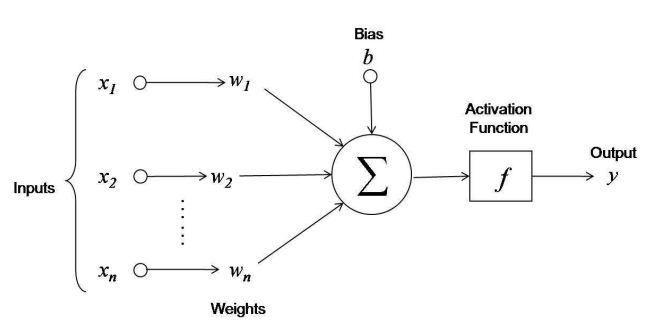
\includegraphics[scale=0.5]{chap3/image/cauTrucMotNoron.jpg}
    \end{center}
    \caption{Cấu trúc của một nơ-ron}
 	\label{fig:aNeural}
    \end{figure}
\end{center}
\par
 Các thành phần cơ bản của nơ-ron:

\begin{enumerate}
\setlength{\itemindent}{5mm}
	\item \textit{Đầu vào} (\textit{x}): các tín hiệu vào của nơ-ron, các tín hiệu này thường đưa vào dưới dạng một vector N chiều và được kí hiệu là $\textbf{x}$ và mỗi phần tử trong vector được kí hiệu là $x_i, i\in{0,n}$
	\item \textit{Trọng số} (\textit{w}): mỗi liên kết được thể hiện bởi một trọng số liên kết và được gọi là weight. Trọng số liên kết giữa tín hiệu vào thứ j với nơ-ron k thường được kí hiệu là $w_{kj}$, và. Thông thường, các trọng số này được khởi tạo một cách ngẫu nhiên theo phân phối chuẩn ở thời điểm khởi tạo mạng và được cập nhật liên tục trong quá trình học mạng.

	\item \textit{Bias (b)}: là tham số nhằm tăng khả năng thích ứng của mạng nơron trong quá trình học. Bias gần giống như trọng số, trừ một điều là nó luôn có tín hiệu vào không đổi bằng 1 (được trình bày rõ hơn ở phần \ref{subsec:feedforward} ). Tham số này có thể bỏ đi nếu không cần thiết.	
	
	\item \textit{Hàm kết hợp  (z)}: Mỗi một đơn vị trong một mạng kết hợp các giá trị đưa vào nó thông qua các liên kết với các đơn vị khác, sinh ra một giá trị gọi là net input. Hàm thực hiện nhiệm vụ này  gọi là hàm kết hợp (combination function), được định nghĩa bởi một luật lan truyền cụ thể. Thông thường hàm này sẽ là hàm tổng của tích các trọng số với đầu vào và độ lệch. Và được biể diễn thông qua biểu thức $z = \sum_{i=1}^n(x_iw_i) +b$.
	\item \textit{Hàm truyền (activiation function hoặc transfer function)}: Hàm này được dùng để giới hạn phạm vi đầu ra của mỗi nơ-ron và nhận đầu vào là kết quả của hàm kết hợp. Tôi sẽ trình bày phần này rõ hơn ở phần \ref{sec:activationFunc}.
	\item \textit{Đầu ra (output)}: Là tín hiệu đầu ra của một nơ-ron, với mỗi nơ-ron sẽ có tối đa là một đầu ra. Nếu như nơ-ron đó ở các hidden layer thì đầu ra của nó được gọi là activation và được kí hiệu là $a$.
\end{enumerate} \par
Khi quy về toán học thì một nơ-ron sẽ được thể hiện thông qua hai hàm sau:
\begin{center}
$z = \sum_{i=1}^n(x_iw_i)+b = \textbf{x}\textbf{w}+b$\\[5pt]
$a = f(z)$
\end{center}
trong đó:
\begin{itemize}
\setlength{\itemindent}{5mm}
	\item[\textendash] $x_i,w_i$ là giá trị thứ $i$ của đầu vào và trọng số tương ứng
	\item[\textendash] Hàm $f$ là hàm truyền và có đầu vào là giá trị của bộ tổng $z$
	\item[\textendash] $a$ là giá trị được tính bởi hàm truyền và là đầu ra của nơ-ron
\end{itemize}
\par
Như vậy một nơ-ron nhận các đầu vào sau đó kết hợp với các trọng số rồi đưa kết quả vào hàm truyền và cho ra một giá trị đầu ra.

\subsection{Cấu trúc của mạng nơ-ron}

\subsubsection{Layer}
\hspace{5mm} Mạng neural  được chia làm 3 lớp chính: lớp đầu vào (\textit{input layer}, màu vàng), lớp ẩn (\textit{hidden layer}, màu xanh lá), lớp đầu ra (\textit{output layer}, màu xanh dương) và trong mỗi lớp có số lượng \textit{unit} khác nhau. Cấu trúc mạng được minh họa trong Hình \ref{fig:neuralNetworkStruct}.
\begin{center}
 	\begin{figure}[htp]
    \begin{center}
     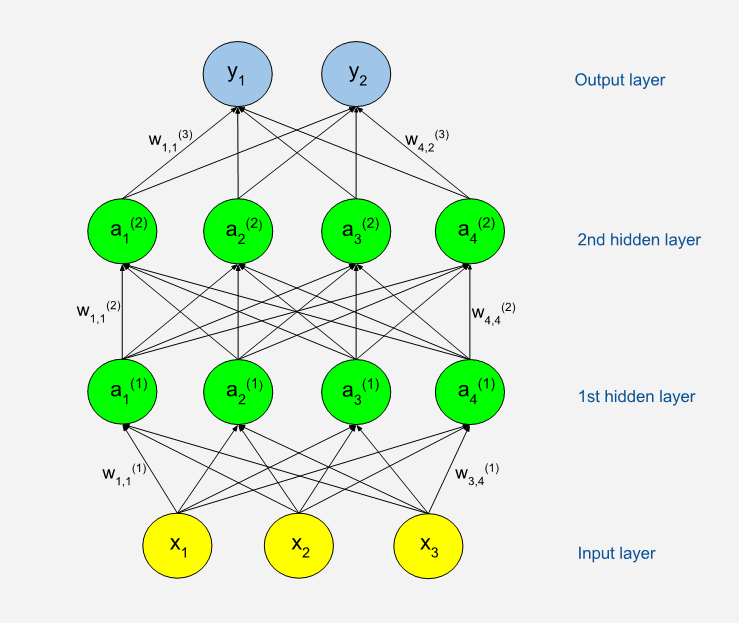
\includegraphics[scale=0.5]{chap3/image/cautrucNN.png}
    \end{center}
    \caption{Cấu trúc mạng nơ-ron}
    \label{fig:neuralNetworkStruct}
    \end{figure}
\end{center}

\begin{itemize}
\setlength{\itemindent}{5mm}
	\item \textit{Input layer}: Biểu diễn tổng quát của mỗi quan sát
	\item \textit{Output layer}: Thể hiện đầu ra dự đoán của model
	\item \textit{Hidden layer}: Là lớp thể hiện cấu trúc của mạng nơ-ron. Các \textit{hidden layer} theo thứ tự từ input layer đến output layer được đánh số thứ tự là \textit{hidden layer 1, hidden layer 2,...}.
\end{itemize}\par
Số lượng layer trong một mạng nơ-ron được ký hiệu là $L$ và được tính bằng số hidden layer cộng thêm một. Ví dụ trong Hình \ref{fig:neuralNetworkStruct}, $L=3$.
\subsubsection{Units}
Mỗi \textit{node} hình trong trong Hình \ref{fig:neuralNetworkStruct} được gọi là một \textit{unit} hoặc một nơ-ron. Như tôi đã trình bày cấu trúc của một nơ-ron ở phần \ref{sec:neuralStruct}, đầu vào của một nơ-ron là một hàm kết hợp và đầu ra thông qua một hàm gọi là activiation. Ở mạng nơ-ron thì đầu vào của hidden layer thứ $l$ được ký hiệu là $\textbf{z}^{(l)}$ với $z^{(l)}_i = \textbf{x}\textbf{w}^{(l)}_i$ và đầu ra của mỗi unit được ký hiệu là $\textbf{a}^{(l)}$ với $\textbf{a}^{(l)}= f(\textbf{z}^{(l)})$.\par

	Số lượng unit trong mỗi lớp, số lượng lớp trong mỗi cấu trúc mạng là không xác định. Nó được xây dựng dựa vào kinh nghiệm của người thiết kế mạng hoặc theo các tài liệu đã được công bố. Nếu số lượng lớp quá lớn thì tốc độ tính toán chậm, còn số lượng lớp ít thì độ tin cậy của kết quả không cao. Nếu số node trong các lớp lớn thì sẽ bị overfitting, ngược lại sẽ bị underfitting. Tôi sẽ trình bày phần overfitting, underfitting ở phần sau.
\subsection{Hàm truyền (activation function)}
\label{sec:activationFunc}
\hspace{5mm} Phần lớn các đơn vị trong mạng nơron chuyển net input  bằng cách sử dụng một hàm vô hướng (scalar-to-scalar function) gọi là hàm kích hoạt, kết quả của hàm này là một giá trị gọi là mức độ kích hoạt của đơn vị (unit's activation). Loại trừ khả năng đơn vị đó thuộc lớp ra, giá trị kích hoạt được đưa vào một hay nhiều đơn vị khác. Các hàm kích hoạt thường bị ép vào một khoảng giá trị xác định, do đó thường được gọi là các hàm bẹp (squashing). Một số hàm thường được sử dụng là ReLU, sigmoid, softmax.
	\subsubsection{Hàm ReLU}
	\label{sec:relu}
\hspace{5mm} Hàm ReLU (Rectified Linear Unit) được sử dụng rộng rãi gần đây vì tính đơn giản của nó. Nó có công thức toán học  $f(s)=\max(0,s)$. Đồ thị hàm ReLU được thể hiện ở Hình \ref{fig:relu}
\begin{center}
 	\begin{figure}[htp]
    \begin{center}
    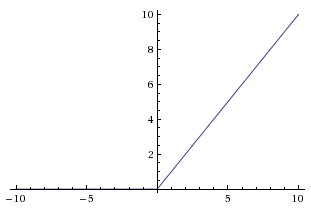
\includegraphics[scale=1]{chap3/image/relu.jpeg}
    \end{center}
    \caption{Hàm ReLU}
    \label{fig:relu}
    \end{figure}
\end{center}
	Từ biểu đồ ta có thể dễ dàng thấy độ lệch của hàm ReLU luôn bằng 1 khi $x>0$, bằng 0 khi $x<0$ và ta quy ước tại  $x=0$ thì độ lệch bằng 0 nhưng trường hợp này rất ít khi xảy ra.\\
	
\begin{center}
	$\frac{d}{dx}ReLU(x) =
    \begin{cases}
       0,$ if $x < 0,\\
       1,  otherwise.
    \end{cases}
    $
\end{center}
	\hspace{5mm} Hàm ReLU thường được sử dụng làm hàm truyền trong các hidden layer, còn ở layer cuối cùng thì ta sẽ sử dụng hàm khác để có thể tính toán được sắc xuất dự đoán vào vùng phân loại.

\subsubsection{ Hàm sigmoid}
	 \hspace{5mm} Hàm logistic là mô hình một dạng đường cong-S của sự tăng trưởng của một tập $P$ nào đó. Sự tăng trưởng được mô hình như sau: giai đoạn tăng trưởng ban đầu được xấp xỉ hàm mũ và khi quá trình bão hòa bắt đầu, sự phát triển sẽ chậm lại, và tới giai đoạn trưởng thành thì dừng hẳn. \par 
	 Hàm logistic có công thức toán học là: 
	 \begin{center}
	 	$P(x,a,m,n,r) = a\frac{1+m\exp({-x/r})}{1+n\exp({-x/r})}$ \rule{5mm}{0pt} với $a,m,n,r$ là các tham số thực.
	 \end{center}
	 \par
	  Hàm sigmoid là một trường hợp đặc biệt của hàm logistic và có công thức toán học là $\sigma(x) = \frac{1}{1+\exp({-t})}$, đồ thị được thể hiện ở Hình \ref{fig:sigmoid}
\begin{center}
 	\begin{figure}[htp]
    \begin{center}
    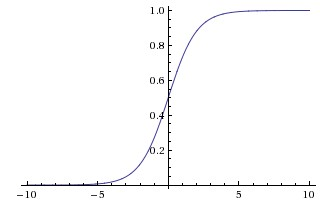
\includegraphics[scale=1]{chap3/image/sigmoid.jpeg}
    \end{center}
    \caption{Hàm sigmoid}
    \label{fig:sigmoid}
    \end{figure}
\end{center}
\hspace{5mm} Nhìn vào đồ thị ta có thể thấy giá trị của hàm nằm trong khoảng (0,1]. Cụ thể, với đầu vào lớn hàm số sẽ cho đầu ra gần với 1 còn với đầu vào nhỏ hàm số sẽ cho đầu ra gần với 0. Hàm số này được sử dụng nhiều trong quá khứ vì có đạo hàm $\frac{d\sigma(x)}{d(x)} = \sigma(x).(1-\sigma(x)$ rất đẹp. Những năm gần đây, hàm số này ít khi được sử dụng do khi có đầu vào là những số cực lớn hoặc cực bé thì đạo hàm của hàm số xấp xỉ bằng 0, điều này gây ảnh hưởng đến việc cập nhập các trọng số trong quá trình học và làm cho thời gian tính toán lâu hơn. Tôi sẽ trình bày tại sao lại như vậy ở phần backpropagation.
	
	\subsubsection{Hàm softmax}
	\label{sec:softmax}
	\hspace{5mm} Hàm softmax hay hàm trung bình mũ là sự khái quát hóa của hàm logistic biến không gian K-chiều véc tơ  với giá trị thực bất kỳ đến không gian K-chiều véc tơ  mang giá trị trong phạm vi (0, 1).\par

Hàm softmax có phương trình toán học như sau:
\begin{center}
	$y_i=\frac{\exp({x_i})}{\sum^{n}_{j=1}{\exp({x_j})}}; \forall i=1,...,n$ %\rule{5mm}{0pt} %
	
	
\end{center}	
với $n$ là số lượng phần tử trong vector \textbf{x}.\par
Hiện nay hàm này được sử dụng rộng rãi trong việc phân loại trong lớp đầu ra. Vì nếu tại giá trị phần tử $x_i$ lớn vượt trội so với toàn bộ dữ liệu ở vector $\textbf{x}$ thì giá trị đầu ra $y_i$ cũng sẽ lớn vượt trội so với đầu ra ở các phần tử khác. Điều tiếp theo chúng ta có thể thấy rằng tổng đầu ra sẽ luôn bằng môt, softmax đã sử dụng hàm $\exp(x)=e^{x}$ (Hình \ref{fig:hamex}) giúp cho giá trị của đầu ra luôn dương và thứ tự các phần tử đầu ra tương ứng với thứ tự đầu vào.
\begin{center}
	\begin{figure}[htp]
	\begin{center}
		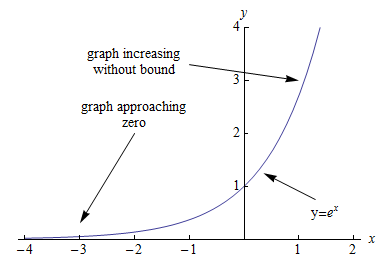
\includegraphics[scale=1]{chap3/image/expgraph.png}
	\end{center}			
	\caption{Đồ thị hàm $f(x)=\exp(x)$}
	\label{fig:hamex}
	\end{figure}
\end{center}

Một vài ví dụ về hàm softmax, với dữ liệu đầu vào là vector \textbf{z} và giá trị đầu ra là vector \textbf{a}, giá trị các vector được thể hiện qua Hình \ref{fig:vdsoftmax}.
\begin{center}
	\begin{figure}[htp]
	\begin{center}
		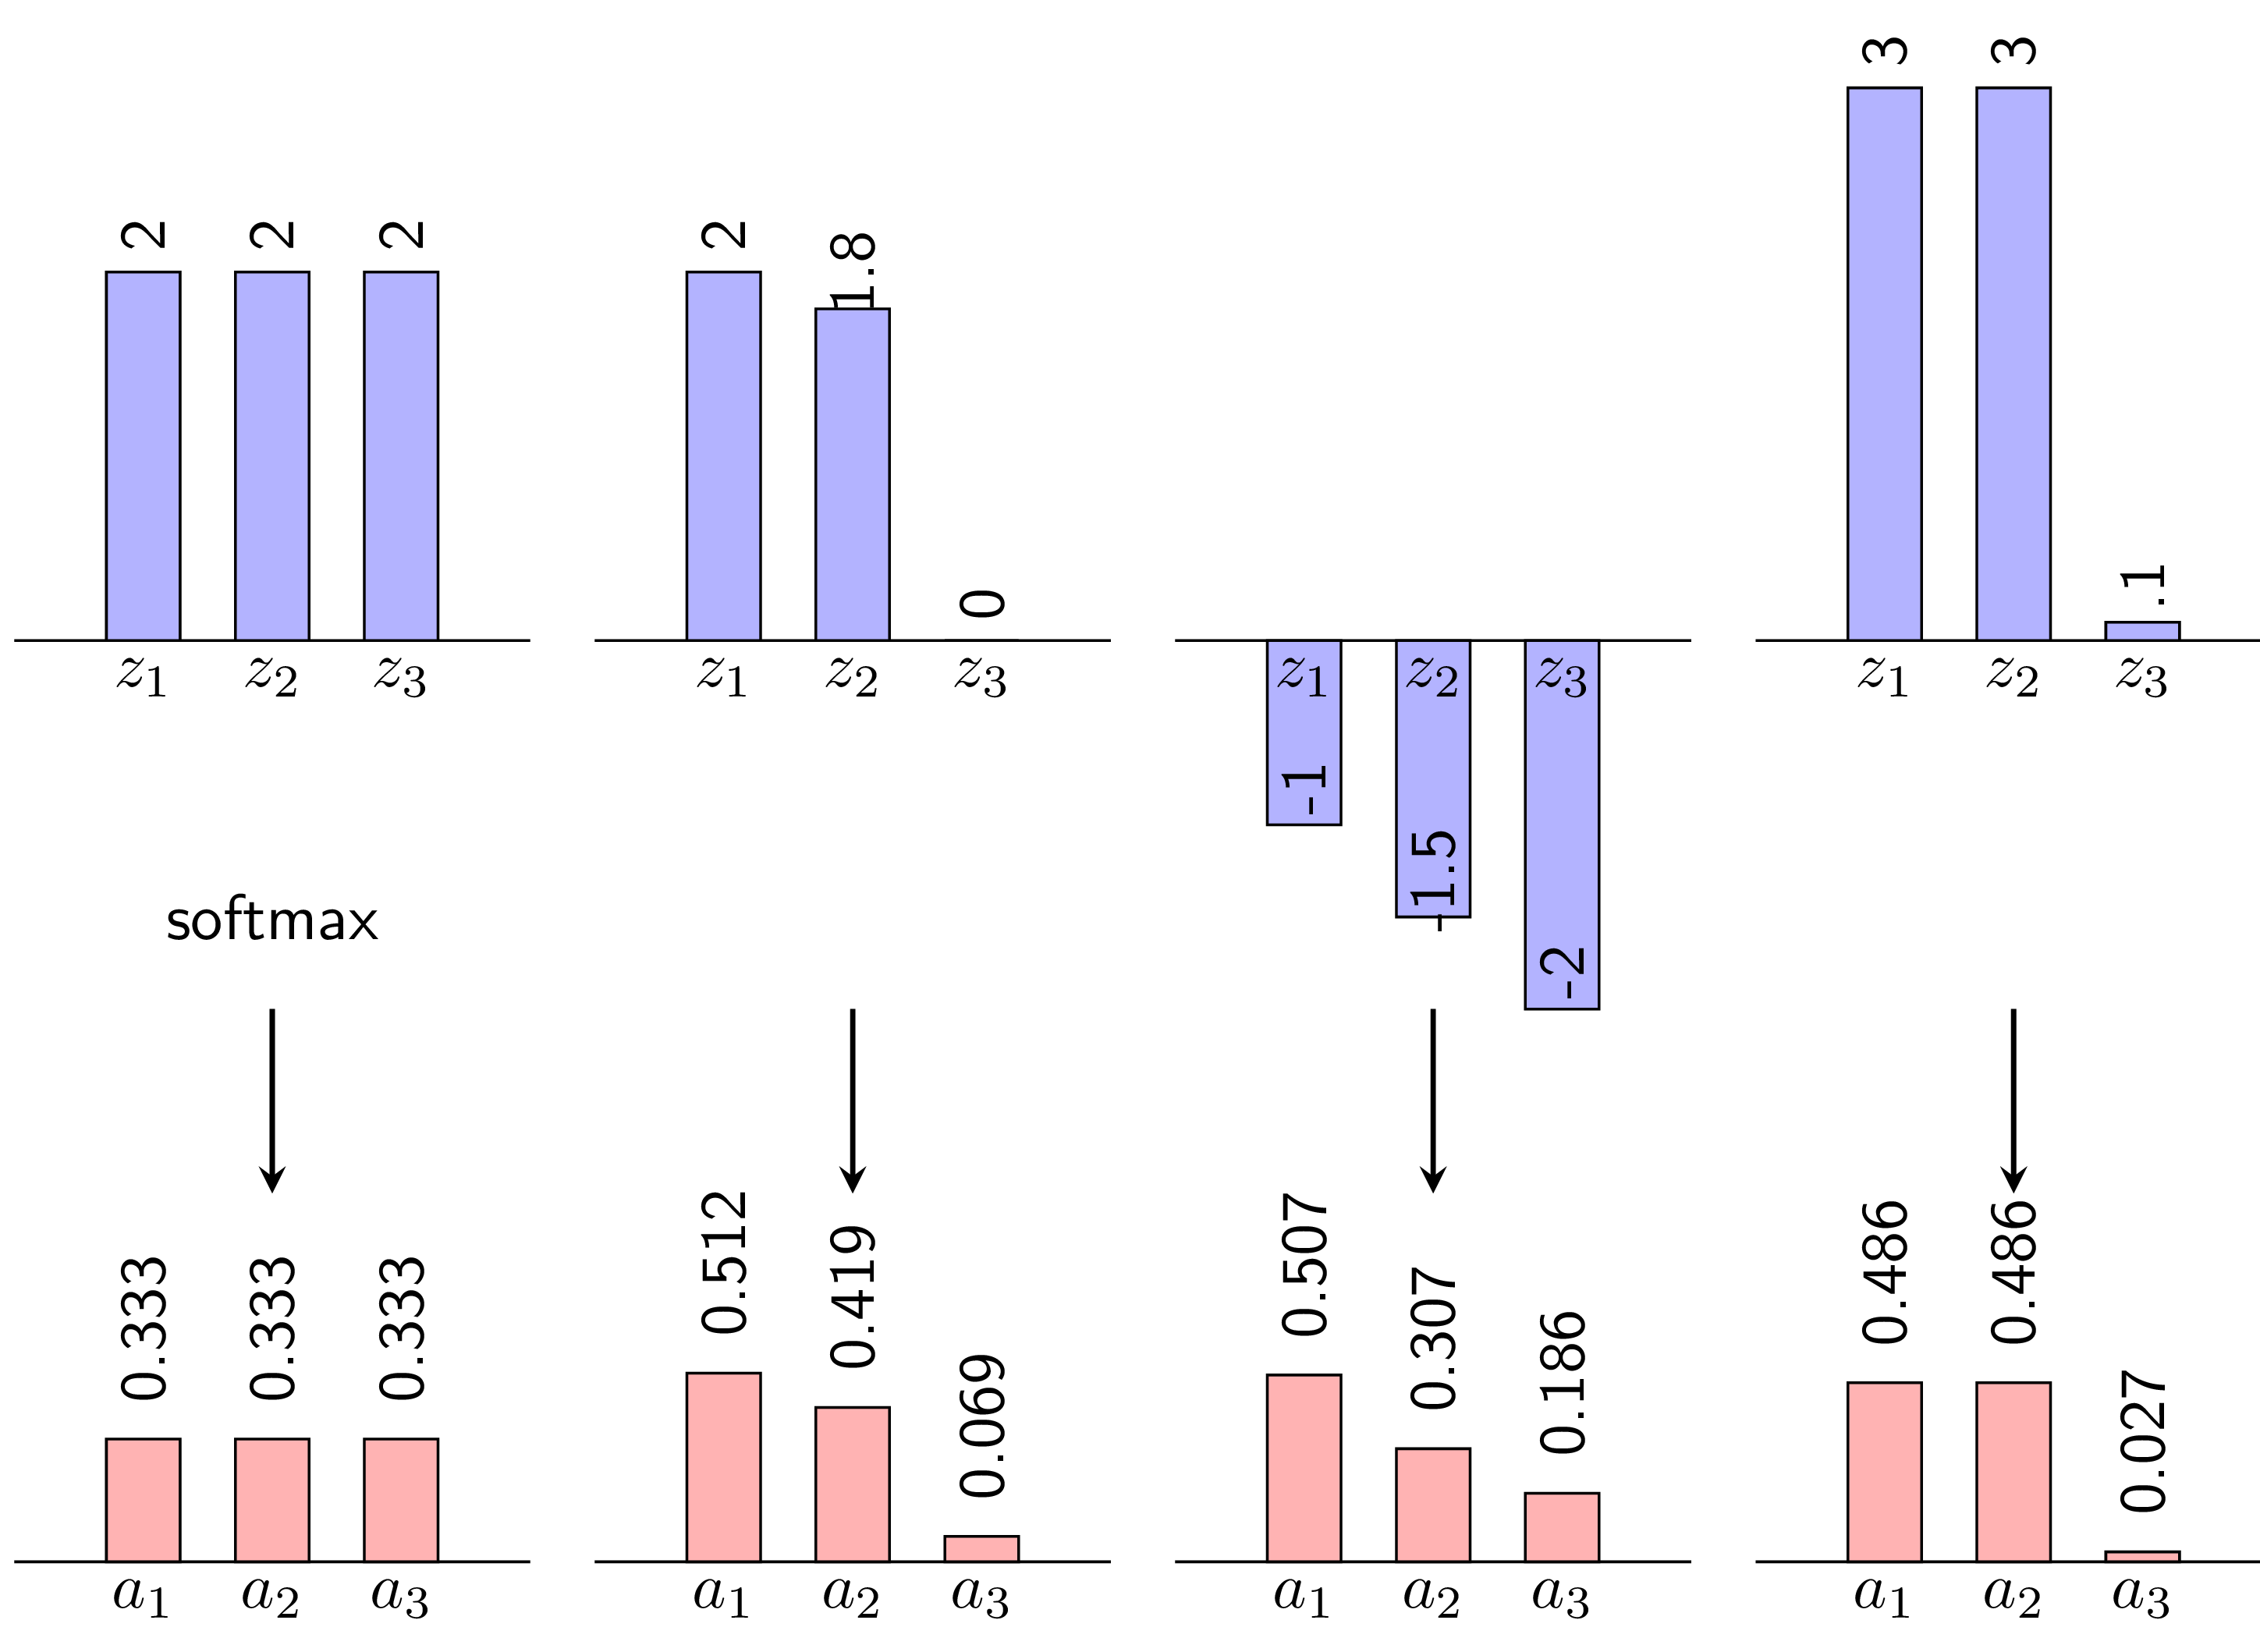
\includegraphics[scale=0.1]{chap3/image/softmax_ex.png}
	\end{center}			
	\caption{Ví dụ hàm softmax}
	\label{fig:vdsoftmax}
	\end{figure}
\end{center}
Tại đây chúng ta có thể thấy giá trị của đầu ra luôn dương, giá trị đầu ra lớn nhất tại giá trị ở phần tử đầu vào lớn nhất, tổng các giá trị đầu ra luông bằng 1. \par

Như vậy với hàm softmax chúng ta có với mỗi đầu ra \textit{$y_i$} luôn phụ thuộc vào tất cả \textit{$x_i$} và đầu ra luôn dương, tổng đầu ra bằng một, thứ tự đầu vào tương ứng với đầu ra. Vì thế  đầu ra $y_i$ có thể coi là xắc suất để đầu vào $x_i$ rơi vào lớp thứ $i$.

\subsection{Mạng lan truyền thẳng}
\label{sec:forward}
%\subsubsection{Truyền thẳng}
%Truyền thẳng là ta tính giá trị đầu ra thông qua các đầu vào cho trước theo thứ tự tính toán trong toán học. 
%Để rõ ràng hơn tôi sẽ trình bày thông qua một ví dụ đơn giản.\par
%Giả sử chúng ta cần tính giá trị hàm  $f(x,y,z) = (x+y)*z$ với $x=-2,y=5,z=-4.$
%Với dữ liệu trên thì ta có thể tính toán đơn giản thông qua phép cộng, nhân và theo thứ tự là trong ngoặc trước, ngoài ngoặc sau. Chúng ta sẽ xây dựng biểu thức trên  một đồ thị với đỉnh là các toán tử (cộng, trừ, nhân, chia, mũ, logarit ...) và lá là các phần tử tham gia đến việc tính toán của đỉnh, đồ thị được thể hiện thông qua Hình \ref{fig:dothi}.
%\begin{center}
%    \begin{figure}[H]
%    \begin{center}
%     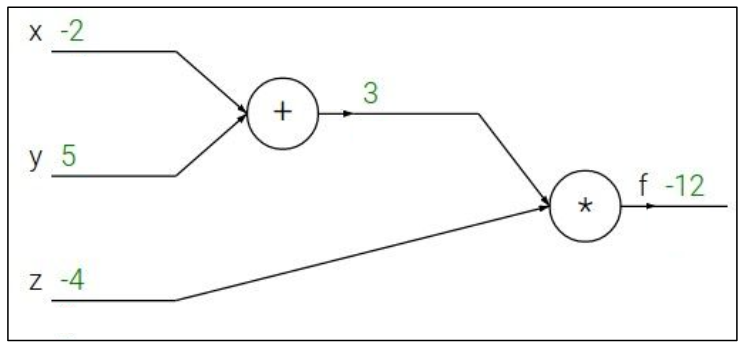
\includegraphics[scale=1]{chap3/image/graph_fw_bp.png}
%    \end{center}
%    \caption{Đồ thị tính toán}
%    \label{fig:dothi}
%    \end{figure}
%\end{center}
%
%Chúng ta sẽ tính hàm $f(x,y,z)$ theo thứ tự của đồ thị. Giả sử ta đặt $q$ là tổng của $x,y$, như vậy để tính được giá trị của hàm $f$ ta cần tính giá trị của tổng $q$ sau đó nhân với giá trị của $z$.
%\begin{enumerate}
%	\item Tính tổng q $q= x+y = -2+5 =3$
%	\item Giá trị của hàm $f=q*z=3*4=12$
%\end{enumerate}
%Với cách tính trên ta gọi đó là truyền thẳng vì nó tính lần lượt và theo thứ tự xác định.
%\subsubsection{Lan Truyền thẳng trong mạng neural}
\subsubsection{Ví dụ}
\hspace{5mm} Giả sử ta có mạng neural như Hình \ref{fig:baitoan} với tập dữ liệu đầu vào là ma trận $\textbf{X}_{2{\times}N}$ ($N$ là số lượng quan sát, 2 là số lượng feature), và label tương ứng là vector $\textbf{y}_{N\times 1}$ (2 là số lượng nhãn), $\textbf{y}_i \in (1,2,3,\ldots,C)$ với C là số lớp cần phân loại .

\begin{figure}[H]
\begin{center}
	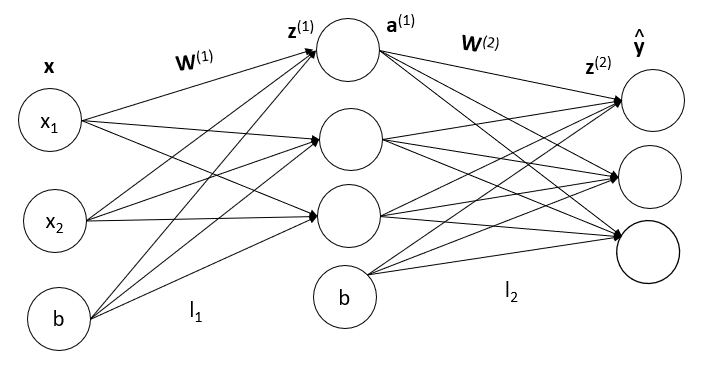
\includegraphics[scale=1]{chap3/image/myNeuralNetwork.png}
	\caption{Mạng neural cho bài toán }
	\label{fig:baitoan}
\end{center}
\end{figure}


Xét một cặp dữ liệu $(\textbf{x}_i,\textbf{y}_i)$ với hàm activation ở hidden layer là hàm relu, hàm activation ở output layer là hàm softmax. Mạng lan truyền thẳng sẽ được tính như sau:

\begin{eqnarray}
\textbf{x}_{1\times 2} &=&\begin{bmatrix} x_1 &x_2 \end{bmatrix} \textbf{W}^{(1)T}_{3{\times}2}  =\begin{bmatrix}
	w^{(1)}_{11} &w^{(1)}_{12} \\[6pt]
	w^{(1)}_{21} &w^{(1)}_{22} \\[6pt]
	w^{(1)}_{31} &w^{(1)}_{32} 
\end{bmatrix}^{T} \label{eq:s1}\\
\textbf{z}^{(1)}_{1 \times 3} &=&	\textbf{x}_{1\times 2}\textbf{W}^{(1)T}_{3\times 2} +b^{(1)}	= \begin{bmatrix}
z^{(1)}_{1} &z^{(1)}_{2} &z^{(1)}_{3} 
\end{bmatrix} \label{eq:s2}	\\
\label{eq:s3}
\textbf{a}^{(1)}_{1 \times 3}	&=&		\max(0,\textbf{z}^{(1)} =	\begin{bmatrix}
	a^{(1)}_1 &a^{(1)}_2 &a^{(1)}_3 
	\end{bmatrix}\\
\label{eq:s4}
\textbf{W}^{(2)T}_{3{\times}3}  &=&	 \begin{bmatrix}
	w^{(2)}_{11} &w^{(2)}_{11} & w^{(2)}_{13}\\[6pt]
	w^{(2)}_{21} &w^{(2)}_{22} & w^{(2)}_{23}\\[6pt]
	w^{(2)}_{31} &w^{(2)}_{32} & w^{(2)}_{33}
\end{bmatrix}^T  \\
\label{eq:s5}
\textbf{z}^{(2)}_{1\times 3}	&=&\textbf{a}^{(1)}_{1 \times 3}\textbf{W}^{(2)T}_{3{{\times}}3}+b^{(2)}	= \begin{bmatrix}
z^{(2)}_{1} &z^{(2)}_{2} &z^{(2)}_{3} 
\end{bmatrix}\\
\label{eq:s6}
\widehat{\textbf{y}}&=&\textbf{a}^{(2)}_{1\times 3} 	= \frac{\exp({\textbf{z}^{(2)}})}{\sum^{2}_{j=1}{\exp({\textbf{z}^{(3)}_j})}}
\end{eqnarray}


Tại các biểu thức số \ref{eq:s1},\ref{eq:s4} là giá trị đầu vào và khởi tạo ma trận trọng số cho layer thứ 1,2; tại biểu thức số \ref{eq:s2},\ref{eq:s5} ta tính giá trị hàm kết hợp (bộ tổng) làm input đầu vào cho nơ-ron; tại biểu thức số \ref{eq:s3},\ref{eq:s6} ta tính đầu ra cho mỗi nơ-ron. Ở layer thứ nhất đầu ra nơ-ron sử dụng \textit{hàm ReLU} \ref{fig:relu} làm hàm activation vì thế tại biểu thứ số \ref{eq:s3} ta có  $\textbf{a}^{(1)}_{1 \times 3}	=\max(0,\textbf{z}^{(1)})$ còn tại layer thứ hai sử dụng hàm softmax làm hàm đầu ra cho nơ-ron nên ta có $\textbf{a}^{(2)}_{1\times 3} = \frac{\exp({\textbf{z}^{(2)}})}{\sum^{3}_{j=1}{\exp({\textbf{z}^{(2)}_j})}}$.


Với tập dữ liệu $(\textbf{X},\textbf{y} )$ thì ta có đầu ra dự đoán như sau:  
\begin{center}

	$\widehat{\textbf{Y}} =\frac{\exp({\textbf{z}^{(2)}_i})}{\sum^{2}_{j=1}{\exp({\textbf{z}^{(2)}_{ij}})}}$; với $i=1,2,...,N$ 

\end{center}
Việc tính toán tuần tự như vậy được được gọi là \textit{feedforward}.
\subsubsection{ Thuật toán}
\label{subsec:feedforward}
\hspace{5mm} Nếu ta thêm một phần tử vào $\textbf{x}_i$ với giá trị bằng 1 và ta coi $b^{(l)}$ là một phần tử của ma trận trọng số $\textbf{W}^{(l)}$ tương ứng với $l$ là layer thứ $l$. Khi đó ta sẽ có công thức tổng quát hơn.

\begin{eqnarray*}
\textbf{a}^{(0)}	&=&		\textbf{x}_i = \begin{bmatrix}
1,x_1,x_2,\ldots,x_n
\end{bmatrix} \\
\textbf{w}^{(l)T}_j &=& \begin{bmatrix}
w^{l}_{j0} := b^{(l)}, w^{l}_{j1}, w^{l}_{j2},\ldots, w^{l}_{jn}
\end{bmatrix}^T\\
\textbf{z}^{(l)}_j &=& \textbf{a}^{(l-1)}\textbf{w}^{(l)}_j\\
\textbf{a}^{(l)} &=& \begin{bmatrix}
1, f(\textbf{z}^{(l)})
\end{bmatrix}^T
\end{eqnarray*}



\begin{algorithm}[H]
\caption{Forward propagation }\label{al:forward}
\begin{algorithmic}[1]
\REQUIRE Network depth, $L$
\REQUIRE $\textbf{W}^{(i)}, i \in \{1,\ldots,L\}$, ma trận trọng số của layer thứ $i$ của model

\REQUIRE $\textbf{X}, \textbf{x}_i, i \in \{1,\ldots,N\} $, tập dữ liệu đầu vào với $n$ là số lượng dữ liệu.
\FOR {$j=1,\ldots,N$}
	
	\STATE $\textbf{a}^{(0)} = \textbf{x}_j$
	\FOR {$i=1,\ldots,L$}
		\STATE $\textbf{z}^{i}=\textbf{a}^{(i-1)} \textbf{W}^{(i)T}$
		\STATE $\textbf{a}^{(i)}=f(\textbf{z}^{(i)})$
\ENDFOR
\STATE $\widehat{\textbf{y}} = \textbf{a}^{(L)}$
\ENDFOR
\end{algorithmic}
\end{algorithm}

%\item Ví dụ\\
%Tiếp tục với vị dụ tại phần Mạng lan truyền thẳng \ref{sec:forward}, ta đi tìm các đạo hàm riêng của từng biến, có nghĩa là đi tìm  $\frac{\partial f}{\partial x}, \frac{\partial f}{\partial y}, \frac{\partial f}{\partial z}$.\par
%Đặt $q=x+y$ khi đó $f=qz$, ta sẽ dễ dàng tính được $\frac{\partial q}{\partial x} =1$, $\frac{\partial q}{\partial y} =1$, $\frac{\partial f}{\partial z} =q=3$, $\frac{\partial f}{\partial q} =z=4$,$\frac{\partial f}{\partial f} =1$.
%
%\begin{center}
%    \begin{figure}[H]
%    \begin{center}
%     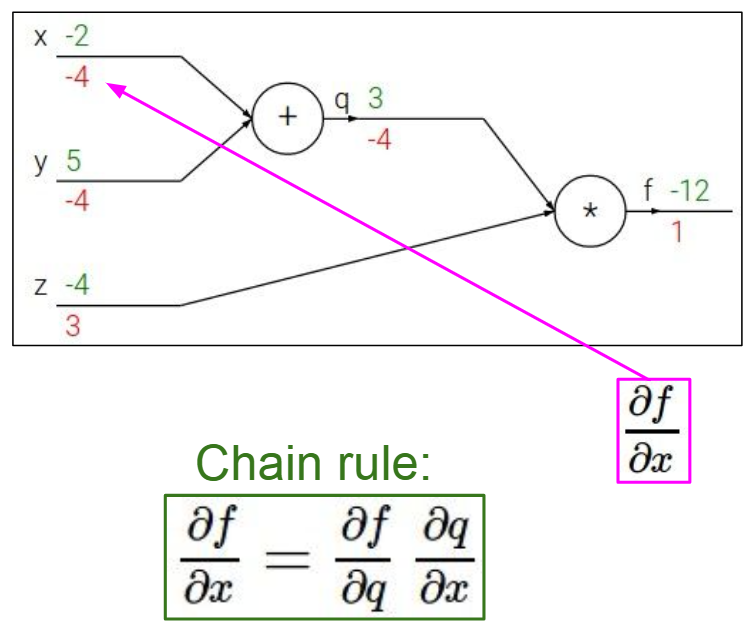
\includegraphics[scale=.5]{chap3/image/backpropagation.png}
%    \end{center}
%    \caption{Backpropagation}
%    
%    \end{figure}
%\end{center}
%\begin{itemize}
%	\item $\frac{\partial f}{\partial z} = \frac{\partial f}{\partial f} \frac{\partial f}{\partial z} = 1*3 = 3$
%	\item $\frac{\partial f}{\partial q} = \frac{\partial f}{\partial f} \frac{\partial f}{\partial q} = 1*4 = 4$
%	\item $\frac{\partial f}{\partial x} = \frac{\partial f}{\partial f}\frac{\partial f}{\partial q} \frac{\partial q}{\partial x} = 1*4*1 = 4$
%	\item $\frac{\partial f}{\partial y} = \frac{\partial f}{\partial f}\frac{\partial f}{\partial q} \frac{\partial q}{\partial y} = 1*4*1 = 4$
%\end{itemize} \par
%Việc tìm đạo hàm riêng của các hàm $f$ theo từng biến, nói cách khác là tìm sự thay đổi của biến khi đầu ra thay đổi, làm như vậy được gọi là truyền ngược (backpropagation).

\subsection{Hàm mất mát và Cross-entropy}
\subsubsection{One-hot encoding}
\hspace{5mm} One-hot encoding là biến mỗi nhãn thành một vector có kích thước bằng với tập nhãn và vị trí nhãn sẽ bằng 1 còn các vị trí còn lại sẽ bằng 0. One-hot encoding được mô tả ở Hình \ref{fig:onehot}. Số lớp cần phần loại gồm: red, yellow, green, blue; các nhãn sẽ được biểu diễn lại như bảng bên; với cột là tập nhãn, dòng là dữ liệu được biểu diễn dưới dạng one-hot encoding.
\begin{figure}[H]
\begin{center}
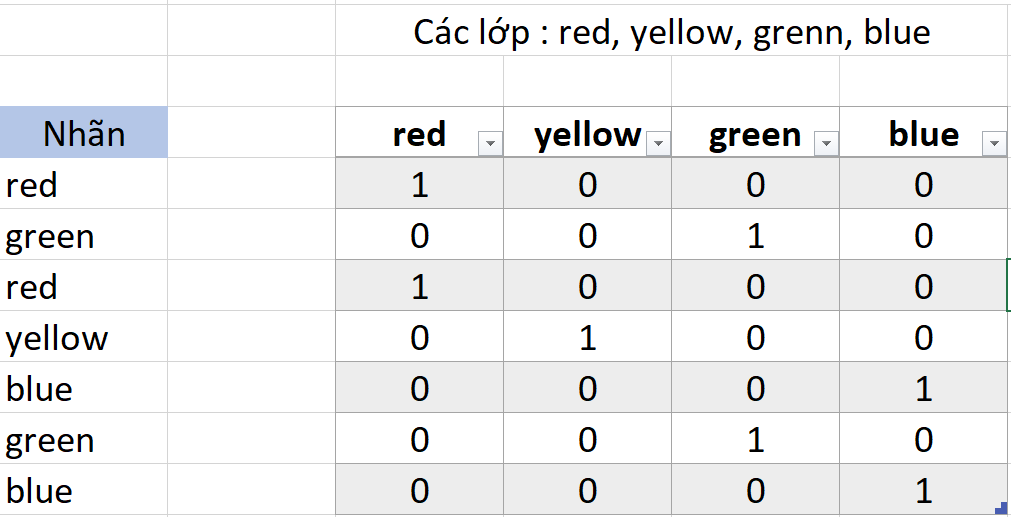
\includegraphics[scale=0.75]{chap3/image/onehot.png}

\caption{ Ví dụ one-hot encoding}
\label{fig:onehot}
\end{center}
\end{figure}
\subsubsection{Hàm mất mát}
\hspace{5mm} Hàm mất mát hay còn gọi là \textit{loss function}, là sự chêch lệch, khác biệt giữa đầu ra dự đoán và đầu ra thực tế, có chức năng là đo độ chính xác của đầu ra dự đoán, thường được ký hiệu là $J$. Giả sử ta cần ánh xạ: $\textbf{X}\to \textbf{Y}$,  trong đó \textbf{X} là tập các vấn đề và Y là tập các lời giải tương ứng cho vấn đề đó thì ta cần xây dựng. Ta cần xây dựng hàm sao cho $\widehat{\textbf{Y}}$ =$ f(\textbf{X},\textbf{W}) \approx \textbf{Y}$. Như vậy hàm mất mát là độ chênh lệch, sự khác biệt giữa \textbf{$\widehat{\textbf{Y}}$} và $\textbf{Y}$. Nếu như giá trị mất mát càng lớn thì điều đó có nghĩa rằng đầu ra dự đoán càng sai, các tham số truyền vào chưa chính xác vì thế chúng ta cần điều chỉnh tham số sao cho hàm \textbf{$\widehat{\textbf{Y}}$} càng gần $\textbf{Y}$ càng tốt. Có nghĩa rằng chúng ta cần tìm: $\textbf{W}$=$\arg\min_{\textbf{W}} J$.\par
Trong nhiều bài toán, các mô hình tham số được định nghĩa như một phân phối $p(\textbf{y}|\textbf{x},\textbf{W})$ và sử dụng nguyên lý Maximum-Likelihood, có nghĩa là chúng ta sử dụng cross-entropy giữa $\widehat{\textbf{y}}$ và $\textbf{y}$ như là hàm mất mát. 

\subsubsection{Cross-entropy}
\hspace{5mm} \textit{Cross entropy} là một đại lượng phản ánh mức độ khác biệt giữa hai phân phối xắc xuất. Sự khác biệt giữa phân bố $p$ và $q$ càng lớn, thì cross-entropy của $p$ đối với $q$ sẽ càng lớn hơn entropy của p.\par 
Cross entropy giữa hai vector phân phối \textbf{p} và \textbf{q} được định nghĩa là:
\begin{equation}
\label{eqn:cross1}
H(\textbf{p},\textbf{q}) = \textbf{E}_\textbf{p}[-\log(\textbf{q})]
\end{equation}\par
	Với $\textbf{p},\textbf{q} $ là rời rạc, công thức \ref{eqn:cross1} được viết dưới dạng:
\begin{equation}
\label{eqn:cross2}
H(\textbf{p}, \textbf{q}) =-\sum_{i=1}^C p_i \log q_i 
\end{equation}\par

\textbf{Chú ý}: Hàm cross entropy không có tính đối xứng $H(\textbf{p}, \textbf{q}) \neq H(\textbf{q}, \textbf{p})$. Theo công thức \ref{eqn:cross1} và \ref{eqn:cross2} chúng ta có thể thấy giá trị của $\textbf{q}$ không thể nhận giá trị là 0. Vì thể khi sử dụng cross entropy trong các bài toán học có giám sát, chúng ta phải để $\textbf{p}$ là đầu ra thực tế vì chỉ có vị trí nhãn là được đánh dấu 1, các vị trí còn lại được đánh dấu 0 (sử dụng one-hot encoding), $\textbf{q}$ là đầu ra dự đoán vì không có xắc suất nào bằng 0 tuyệt đối cả.

\subsubsection{Xây dựng hàm mất mát}
\hspace{5mm} Giả sử số lớp chúng ta cần phân loại là $C$, xét một cặp dữ liệu $(\textbf{x}_i,\textbf{y}_i)$ với $\textbf{y}_i$ là dạng one-hot tại đầu ra thực tế thứ $i$ và đầu ra dự đoán $\widehat{\textbf{y}_i} = softmax(\textbf{a}^{(L)}_i\textbf{W}^{(L)T}_i)$. Như đã trình bày ở phần \ref{sec:softmax}, giá trị $\widehat{\textbf{y}_{ij}}$\textit{ với j=1,...,C} thể hiện xắc suất để $\textbf{x}_i$ rơi vào lớp thứ $j$. Chúng ta coi  hai vector xắc suất $\widehat{\textbf{y}_{i}}$, $\textbf{y}_i$ lần lượt là $\textbf{q},\textbf{p}$ ở trong biểu thức \ref{eqn:cross2} do đó \textit{giá trị mất mát} được tính như sau:
\begin{equation}
\label{eq:cost1}
\begin{split}
J_i(\textbf{W}) = J_i(\textbf{W};\textbf{x}_i,\textbf{y}_i) &=-\sum_{j=1}^C y_{ij} \log \widehat{y}_{ij}	\\
&= -\sum_{j = 1}^C y_{ij}\log\left(\frac{\exp(\textbf{a}^{(L-1)}_i\textbf{w}^{(L)T}_{ij})}{\sum_{k=1}^C \exp(\textbf{a}^{(L-1)}_{i}\textbf{w}^{(L)T}_{ik})}\right)\\
&= -\sum_{j=1}^C\left(y_{ji} \textbf{a}^{(L-1)}_i\textbf{w}^{(L)T}_{ij}\log\left(\sum_{k=1}^C \exp(\textbf{a}^{(L-1)}_i\textbf{w}^{(L)T}_{ik})\right)\right) \\
&= -\sum_{j=1}^C y_{ji} \textbf{a}^{(L-1)}_i\textbf{w}^{(L)T}_{ij} + \log\left(\sum_{k=1}^C \exp(\textbf{a}^{(L-1)}_i\textbf{w}^{(L)T}_{ik})\right) 
\end{split}
\end{equation}
với  $y_{ij}, \widehat{y}_{ij}$ lần lượt là phần tử thứ j của vector đầu ra thực tế (\textit{one-hot}) $\textbf{y}_i$ và vector đầu ra dự đoán $\widehat{\textbf{y}}_i$. \par

Khi dữ liệu là một tập hợp $(\textbf{x}_i,\textbf{y}_i)$, $i=1,2,...,N$ thì hàm mất mát cho \textit{softmax} được tính như sau
\begin{equation}
\label{eq:cost2}
J(\textbf{W};\textbf{X},\textbf{Y}) = -\frac{1}{N} \sum_{i=1}^N \left(  \sum_{j=1}^C y_{ji} \textbf{a}^{(L-1)}_i\textbf{w}^{(L)T}_{ij} + \log\left(\sum_{k=1}^C \exp(\textbf{a}^{(L-1)}_i\textbf{w}^{(L)T}_{ik})\right) \right)
\end{equation} 


\subsubsection{Backpropagation và tối ưu hàm mất mát}
\begin{enumerate}
\item {Khái niệm và mối liên hệ}\\
\hspace{5mm} Truyền ngược (backpropagation) là ta đi tìm đạo hàm của các trọng số theo hàm mát mát hay có nghĩa là tìm sự thay đổi của các trọng số khi giá trị hàm mất mát thay đổi. \par 
\hspace{5mm} Tối ưu hàm mất mát là ta áp dụng các phương pháp tối ưu như gradient descent, gradient descent với momentum, adam,... để cập nhật trọng số sao cho giá trị của hàm mất mát bị giảm đi.\par
\hspace{5mm} Để có thể làm giảm giá trị của hàm mất mát chúng ta cần sử dụng backpropagation để tính toán đầu vào cho các phương pháp tối ưu. Vì thế đôi khi nó còn được gọi là "backward propagation of errors" tức là "truyền ngược của sai số".

\item {Thuật toán}\\
\begin{algorithm}[H]
\caption{Backpropagation kết hợp với tối ưu}
\label{al:backward}
\begin{algorithmic}[1]
\REQUIRE Network depth, $L$
\REQUIRE $\textbf{W}^{(i)}, i \in \{1,\ldots,L \}$, ma trận trọng số của layer thứ $i$ của model
\REQUIRE $\textbf{b}^{(i)}, i \in \{1,\ldots,L \}$, bias layer thứ $i$ của model	
\REQUIRE $\textbf{X}, \textbf{x}_i, i \in \{1,\ldots,n \} $, tập dữ liệu đầu vào với $n$ là số lượng dữ liệu
\REQUIRE $\textbf{Y}$, tập đầu ra tương ứng dạng one-hot; $\textbf{y}_i, i\in \{1,\ldots,N\}$ đầu ra tương ứng với $x_i$

\FOR {$i=1;i\le N;i=i+1 $}
\STATE $\widehat{\textbf{y}} = \textbf{a}^{(l)}= f(\textbf{x}_{i},\textbf{W}_{i},\textbf{b}_{i})$

\STATE	$\textbf{e}^{(L)} = \frac{\partial J(\widehat{\textbf{W}}}{\partial \textbf{z}^{(L)}}$

\STATE $\frac{\partial J(\textbf{W})}{\partial \textbf{w}^{L}_j} = \textbf{e}^{(L)} \frac{\partial \textbf{z}^{(L)}}{\partial \textbf{w}^{(L)}_j} = \textbf{a}^{(L-1)}_{j}\textbf{e}^{(L)}$ , \textit{với mỗi $j$; $j =1,\ldots, m;$} m là số units trong layer L \\
	\FOR {$k=L-1;k \ge 1;k++$}
		\STATE $\textbf{e}^{(k)}= \textbf{e}^{(k+1)} \frac{\partial  {\textbf{z}^{(k+1)}}}{\partial \textbf{a}^{k}} \frac{\partial\textbf{a}^{k}}{\partial\textbf{z}^{k}} $
		\STATE $\frac{\partial J(\textbf{W})}{\partial \textbf{w}^{k}_j}  =\textbf{e}^{(k)} \frac{\partial \textbf{z}^{(k)}}{\partial \textbf{w}^{(k)}_j} = \textbf{a}^{(k-1)}_{j}\textbf{e}^{(k)}$,  \textit{với mỗi $j$; $j =1,\ldots, m;$} m là số units trong layer $k$ \\
		
	\ENDFOR
	\FOR {$k=L;k \ge 1;k++$} % khong cho vao phong for tren duoc do việc cập nhật có liên quan đến w
	\STATE 	\textit{cập nhật }$\textbf{w}^{(k)}_j$ \textit{ theo gradient } $\frac{\partial J(\textbf{W})}{\partial \textbf{w}^{k}_j} $ \textit{ bằng một trong các cách tối ưu như: gradient descent, adam, momentum,... với mỗi $j$; $j =1,\ldots, m$; $m$ là số units trong layer $k$}
	
	\ENDFOR
\ENDFOR
\end{algorithmic}
\end{algorithm}

\item Ví dụ\\
\hspace{5mm} Tiếp tục ví dụ với cấu trúc mạng nơ-ron như Hình \ref{fig:baitoan}, xét một cặp dữ liệu $(\textbf{x}_i,\textbf{y}_i)$ với $\textbf{y}_i$ là dạng \textit{one-hot} tại đầu ra thực tế thứ $i$. Vì ta hiện ta chỉ xét một cặp dữ liệu vì thế tôi xin được lược bỏ chỉ số $i$ tại các công thức dưới đây. Theo như ta tính bằng \textit{feedforward }chúng ta đã có: 
\begin{itemize}
	\item[] $\textbf{a}^{(0)}=\textbf{x}_{1\times2}$
	\item[]  $\textbf{z}^{(1)}_{1 \times 3}=\textbf{a}\textbf{W}^{(1)T}_{2{\times}3}$
	\item[] $\textbf{a}^{(1)}_{1 \times 3}=\max(0,\textbf{z}^{(1)})$
	
	\item[] $\textbf{z}^{(2)}_{1\times 3}=\textbf{a}^{(1)}_{1 \times 3}\textbf{W}^{(2)T}_{3{{\times}}3 }$
	
	\item[] $\widehat{\textbf{y}}_{1\times 3} = \frac{\exp({\textbf{z}^{(2)}})}{\sum^{3}_{j=1}{\exp({\textbf{z}^{(2)}_j})}}$.

\end{itemize}
Để thực hiện thuật toán backpropagation có nghĩa là chúng ta đi tìm các giá trị sau: $\frac{\partial J_i(\textbf{W})}{\partial \textbf{W}^{(2)}},\frac{\partial J_i(\textbf{W})}{\partial \textbf{W}^{(1)}}$. Vì ta sử dụng hàm activation ở layer cuối là softmax vì thế ta có hàm mất mát là được biểu diễn theo biểu thức \ref{eq:cost2}. Vì $J(\textbf{W})=\sum^{C}_{s=1} y_{s}{ \log \widehat{y}_{s}}$. Vì $\frac{\partial J(\textbf{W})}{\partial \textbf{W}} = \left[
\frac{\partial J(\textbf{W})}{\partial \textbf{w}_1}, \frac{\partial J(\textbf{W})}{\partial \textbf{w}_2},...,\frac{\partial J(\textbf{W})}{\partial \textbf{w}_j},...,\frac{\partial J(\textbf{W})}{\partial \textbf{w}_n} \right]$, nên để đơn giản chúng ta sẽ đi tính giá trị con sau đó sẽ tổng quát hóa hay ta đi tính $\frac{\partial J_i(\textbf{W})}{\partial \textbf{w}^{(L)}_j} $, với $L$ thể hiện là lớp cuối cùng và tại đây thì giá trị của $L=2$. 

\begin{equation*}
\begin{split}
e_j^{(L)} &= \frac{\partial J(\textbf{W}) }{\partial \textbf{z}_j^{(L)}} \\
&=-\sum^{C}_{s=1} y_{s}\frac{ \log \widehat{y}_{s}}{\partial \textbf{z}_j^{(L)}} \\
&=-\sum^{C}_{s=1} y_s \frac{1}{\widehat{y}_s}\frac{\partial \widehat{y}_s}{\partial \textbf{z}^L_j}\\
& = - y_{j}\frac{\sum^C_{k=1}\exp{(z^{(L)}_k)}}{\exp{(z^{(L)}_j)}} \frac{\exp(z^{(L)}_j) \sum^C_{k=1}\exp(z^{(L)}_k) - (\exp(z^{(L)}_{j}))^2}{\left(\sum^C_{k=1}\exp(z^{(L)}_k)\right)^2}\\
&~~ - \sum^C_{s\neq j} y_s \frac{1}{\widehat{y}_s}  \frac{0\sum^C_{s=1}\exp(z^{(L)}_s) - \exp(z^{(L)}_{s}\exp(z^{(L)}_{j}} {\left(\sum^C_{k=1}\exp(z^{(L)}_k)\right)^2}\\
&= -y_{j}\left(1-\frac{\exp(z^{(L)}_j)}{\sum^C_{k=1}\exp(z^{(L)}_k)}\right) - \sum^C_{s\neq j} y_s \frac{1}{\widehat{y}_s}\frac{\left(-\exp(z^{(L)}_{s})\exp(z^{(L)}_{j})\right)} {\left(\sum^C_{k=1}\exp(z^{(L)}_k)\right)^2} \\
& = -y_{j} \left( 1-\widehat{y}_j \right) +  \sum^C_{s\neq j}y_s \frac{1}{\widehat{y}_s}	(\widehat{y}_s	\widehat{y}_j)\\
& = \widehat{y}_j\left(\sum_{s=1}^C   y_s\right) -y_{j}\\
& = \widehat{y}_j - y_j ~~~~~~\textit{do đầu ra thực tế dạng one-hot nên tổng của nó luôn bằng 1}
\end{split}
\end{equation*}
Do đó ta có
\begin{equation}
\label{eq:back_gra1}
\begin{split}
\textbf{e}^{(L)} & = \widehat{\textbf{y}} - \textbf{y} = \textbf{a}^{(L)}-\textbf{y}\\
\frac{\partial J_i(\textbf{W})}{\partial \textbf{W}^{(L)}}& = \textbf{a}^{(L-1)}[e_1,e_2,\ldots,e_C]=\textbf{a}^{(L-1)}\textbf{e}^{T}
\end{split}
\end{equation}
Nếu ta tính theo hàm mất mát đã được khai triển ở biểu thức \ref{eq:cost1} thì việc đạo hàm khá đơn giản.
\begin{equation*}
\begin{split}
\frac{\partial J_i(\textbf{W})}{\partial \textbf{w}^{(L)}_j}  
&=\frac{\partial \left( -\sum_{j=1}^C y_{j} \textbf{a}^{(L-1)}\textbf{w}^{(L)T}_{j} + \log\left(\sum_{k=1}^C \exp(\textbf{a}^{(L-1)}_i\textbf{w}^{(L)T}_{j})\right) \right)}{\partial \textbf{w}^{(L)}_j}\\
&=-y_{j}\textbf{a}^{(L-1)} + 
\frac{\exp(\textbf{w}_j^{(L-1)T}\textbf{a}^{(L-1)})}{\sum_{k = 1}^C \exp(\textbf{w}_k^{(L-1)T}\textbf{a}^{(L-1)})}\textbf{a}^{(L-1)} \\
&= -y_{j}\textbf{a}^{(L-1)} + a^{(L)}_{j} \textbf{a}^{(L-1)}= \textbf{a}^{(L-1)} (a^{(L)}_{j} - y_{j})~ \text{với} ~a_j^{(L)} = \widehat{y}_j \\
&= e^{(L)}_{j}\textbf{a}^{(L-1)} ~(\text{với}~ e^{(L)}_{j} = a^{(L)}_{j} - y_{j})
\end{split}
\end{equation*} 
Tổng quát ta có:
\begin{equation}
\frac{\partial J_i(\textbf{W})}{\partial \textbf{W}^{(L)}} = \textbf{a}^{(L-1)}[e_1,e_2,\ldots,e_C]=\textbf{a}^{(L-1)}\textbf{e}^{(2)T}
\end{equation}
Chúng ta có thể thấy cách tính toán trên cũng cho kết quả với kết quả tại biểu thức \ref{eq:back_gra1}, như vậy chúng ta đã có các đạo hàm $\frac{\partial J_i(\textbf{W})}{\partial \textbf{W}^{(2)}}$. Tiếp theo chúng ta sẽ tính $\frac{\partial J_i(\textbf{W})}{\partial \textbf{W}^{(1)}}$.
\begin{eqnarray*}
\frac{\partial J_i(\textbf{W})}{\partial \textbf{w}^{(1)}_j} &=& \textbf{e}^{(L)}\frac{\partial\textbf{z}^{(2)}}{\partial \textbf{a}^{(1)}} \frac{\partial \textbf{a}^{(1)}}{\partial \textbf{z}^{(1)}_j} \frac{\partial \textbf{z}^{(1)}_j}{\partial \textbf{w}^{(1)}_j}  \\
&=&(\textbf{a}^{(2)}-\textbf{y})\textbf{w}^{(2)T}_j 1\textbf{a}^{(0)}\\
&=&\textbf{a}^{(0)}e^{(1)T}
\end{eqnarray*}
Tổng quát hóa ta có:
\begin{equation}
\frac{\partial J_i(\textbf{W})}{\partial \textbf{W}^{(1)}} = (\textbf{a}^{(2)}-\textbf{y})\textbf{W}^{(2)T} 1 \textbf{a}^{(0)} = \textbf{a}^{(0)}\textbf{e}^{(1)T}
\end{equation}
Như vậy với tập dữ liệu $N$ quan sát thì chúng ta có thể như sau:
\begin{equation}
\begin{split}
\frac{\partial J(\textbf{W})}{\partial \textbf{W}^{(2)}} &=\sum^{N}_{i=1} \textbf{a}^{(2-1)}_i\textbf{e}^{(2)T}_i = \textbf{A}^{(2-1)}\textbf{E}^{(2)T}\\
\frac{\partial J(\textbf{W})}{\partial \textbf{W}^{(1)}} &= \sum^{N}_{i=1} \textbf{a}^{(0)}_i \textbf{e}^{(1)T}_i = \textbf{X}\textbf{E}^{(1)T}
\end{split}
\end{equation}
với $\textbf{E}^{(2)} = \textbf{A}^{(2)}-\textbf{Y}, ~ \textbf{E}^{(1)} = \textbf{E}^{(2)}\textbf{W}^{(2)T}$
Bước tiếp theo là sử dụng kết quả vừa tìm được để tối ưu hàm mất mát bằng các phương pháp tối ưu tôi đã trình bày ở phần \ref{sec:toiuu}. Ví dụ tôi chọn phương pháp gradient descent, chúng ta có:
\begin{equation}
\begin{split}
\textbf{E}^{(2)} &= \textbf{A}^{(2)}-\textbf{Y}\\
\textbf{W}^{(2)} &=\textbf{W}^{(2)} + \eta \textbf{A}^{(2-1)}\textbf{E}^{(2)T} \\
 \textbf{E}^{(1)} &= \textbf{E}^{(2)}\textbf{W}^{(2)T}\\
\textbf{W}^{(1)} &= \textbf{W}^{(1)} + \eta \textbf{X}\textbf{E}^{(1)T}\\
\end{split}
\end{equation}


\end{enumerate}
\subsection{Overfitting}
\hspace{5mm} Overfitting là một hiệnn tượng không mong muốn thường gặp trong quá trình xây dựng mô hình, người xây dựng mô hình cần nắm được kỹ thuật để tránh hiện tượng này xảy ra.
\subsubsection{Tổng quan}
\hspace{5mm} Để hiểu vấn đề này chúng ta sẽ cùng nhau xem qua ví dụ sau  Hình \ref{fig:overfitting}.
\begin{center}
 	\begin{figure}[H]
    \begin{center}
    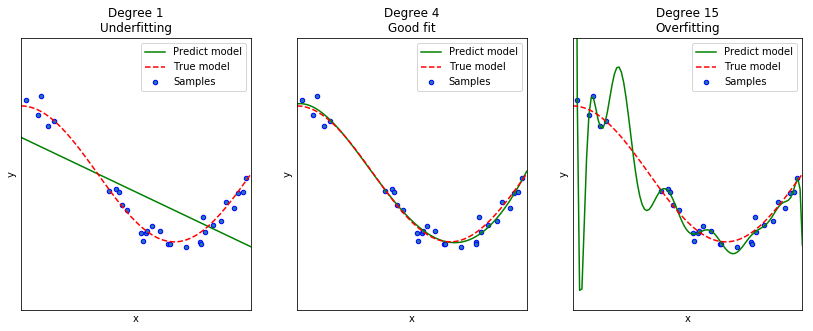
\includegraphics[scale=0.5]{chap3/image/overfitting.png}
    \end{center}
    \caption{overfitting và underfitting}
    \label{fig:overfitting}
    \end{figure}
\end{center}
Đường nét liền thể hiện \textit{mô hình dự đoán (predicted model)} , đường nét đứt thể hiện \textit{mô hình thực (true model)}, các chấm hình tròn là các điểm dữ liệu. Mô hình được xây dựng bằng hồi quy tuyến tính (\textit{linear regression}) với các feature là bậc mũ.\par
Ở hình thứ nhất chúng ta có thể thấy mô hình dự đoán là một hàm tuyến tính (bậc bằng 1) rất khác với mô hình thực, xa với các điểm dữ liệu. Hiện tượng này ta nói mô hình bị \textit{underfitting}.
Với mô hình dự đoán là đa thức bậc 4 chúng ta có thể thấy mô hình dự đoán xấp xỉ như mô hình thực (hình thứ 2). Trường hợp này ta nói mô hình phù hợp (\textit{good fit}). Ở hình thứ 3, khi ta tăng bậc đa thức lên thì mô hình dự đoán quá khớp với các điểm dữ liệu, gần như mọi điểm dữ liệu đều nằm trên mô hình. Tuy nhiên việc khớp hoàn toàn dữ liệu lại không hề tốt vì dữ liệu thường bị nhiễu và có thể khiến mô hình dự đoán bị nhiễu hơn. Trường hợp này ta nói mô hình bị\textit{ overfitting}. Để tránh vấn đề này xả ra chúng ta có hai phương pháp khá là hữu dụng đó là \textit{early stopping} và \textit{regularization}.\\
\textbf{Một vài khái niệm về mô hình}
\begin{enumerate}
\item
\textit{Underfitting} là hiện tượng mô hình chưa được phù hợp với tập dữ liệu huấn luyện và cả các mẫu mới khi dự đoán. Nguyên nhân có thể là do mô hình chưa đủ độ phức tạp cần thiết để bao quát được tập dữ liệu.
\item   \textit{Overfitting} là hiện tượng mô hình quá khớp với \textit{tập dữ liệu huấn luyện (training set)}, việc này sẽ gây ra hậu quả vô cùng nghiêm trọng nếu tập dữ liệu huấn luyện xuất hiện nhiễu. Mô hình sẽ chỉ chú trọng vào việc xấp xỉ với tập dữ liệu huấn luyện mà quên đi mục đích ban đầu là tổng quát hóa, làm cho mô hình sẽ không thật sự tốt dối với dữ liệu nằm ngoài dữ liệu huấn luyện (dữ liệu test và dữ liệu thực tế). Overfitting xảy ra khi \textit{độ phức tạp của mô hình quá lớn} hoặc \textit{quá ít dữ liệu}.
\item \textit{Good fitting} là mô hình nằm giữa 2 mô hình chưa khớp (\textit{underfitting}) và quá khớp (\textit{overfitting}) cho ra kết quả hợp lý với cả tập dữ liệu huấn luyện và các giá trị mới, tức là nó mang được tính tổng quát như hình 1 ở giữa phía trên. Lý tưởng nhất là khớp được với nhiều dữ liệu mẫu và cả các dữ liệu mới. Tuy nhiên trên thực tế được mô hình như vậy rất hiếm.
\end{enumerate}.
\subsubsection{Mối liên hệ giữa overfitting và giá trị hàm mát mát}
\hspace{5mm} Như tôi đã trình bày phần trên, overfitting là hiện tượng mô hình quá khớp với tập dữ liệu huấn luyện có nghĩa là giá trị của hàm mất mát trên tập dữ liệu huấn luyện (\textit{$J_{train}$}) rất nhỏ. Nhưng khi đó giá trị của hàm mất trên tập dữ liệu test (\textit{$J_{test}$}) lại tăng lên gây ra mô hình mất đi sự tổng quát. 

\begin{center}
 	\begin{figure}[H]
    \begin{center}
    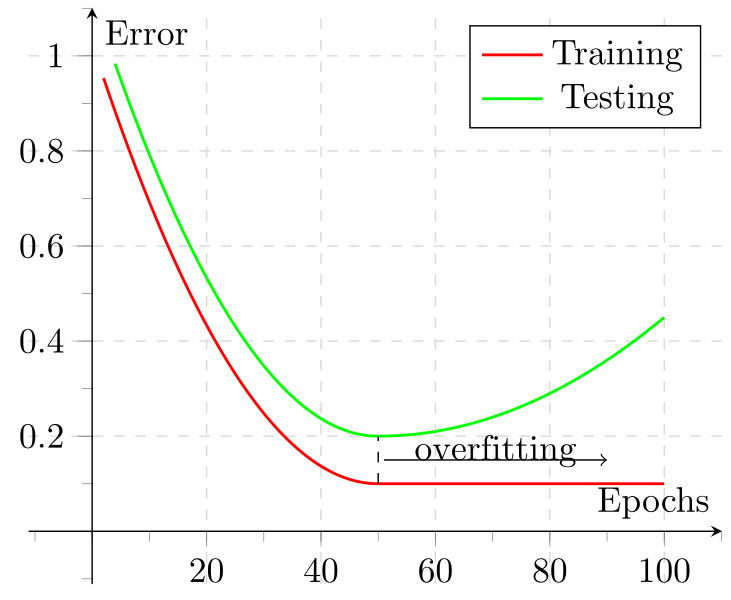
\includegraphics[scale=0.5]{chap3/image/overfittingError.png}
    \end{center}
    \caption{Overfitting xảy ra khi giá trị mất mát giữa tập train giảm còn tập test tăng}
    \label{fig:overfittingError}
    \end{figure}
\end{center}

\subsubsection{Early stopping}
\hspace{5mm} Khi ta dùng một phương pháp tối ưu hàm số để giảm thiểu giá trị mất mát thì \textit{$J_{train}, J_{test}$} sẽ cùng giảm theo thời gian nhưng nếu sau một thời gian \textit{$J_{test}$} tăng lên còn \textit{$J_{train}$} tiếp tục giảm thì đó là lúc bắt đầu dẫn đến overfitting. Cách đơn giản nhất để giảm thiểu overfitting đó là dừng huấn luyện tại ngay thời điểm bắt đầu overfitting và phương pháp này được gọi là \textit{early stopping}. Nếu ta có biểu đồ về sự thay đổi giá trị mất mát của trainning và testing như Hình \ref{fig:overfittingError} thì ta có thể thấy thời điểm sử dụng early stopping là vào khoảng epochs 50.

\subsubsection{Regularization}
\hspace{5mm} \textit{Regularization} là thay đổi mô hình một chút, chấp nhận hy sinh độ chính xác trong trainning set nhưng giảm độ phức tạp của mô hình, do đó giúp tránh được được overfitting mà vẫn giữ được tính tổng quát của mô hình.
\begin{enumerate}
\item Thêm số hạng vào hàm mất mát\\
\hspace{5mm} Một kỹ thuật regulazation phổ biến là thêm một số hạng vào hàm mất mát như sau:
\begin{equation}
	J_{reg}(\textbf{W}) = J(\textbf{W})+ \lambda R(\textbf{W})
\end{equation}
$J(\textbf{W})$ là hàm mất mát ban đầu và cụm $ \lambda R(\textbf{W})$  mới thêm vào là số hạng chính quy hoá (hay số hạng regularization) đóng vai trò như một biện pháp phạt lỗi (penalization).Trong đó, tham số chính quy hoá (\textit{regularizaton parameter}) $\lambda$ được chọn từ trước để cân bằng giữa $J(\textbf{W}) ~\text{và}~ R(\textbf{W})$. $\lambda$ càng lớn thì ta càng coi trọng $R(\textbf{W})$, ít coi trọng tham số cho hàm mất mát ban đầu hơn, dẫn tới việc các trọng số $\textbf{W}$ ít có ảnh hưởng tới mô hình hơn. Hay nói cách khác là mô hình bớt phức tạp đi giúp ta đỡ việc lỗi quá khớp.
$R(\textbf{W})$ thường có dạng như sau:
\begin{equation}
R(\textbf{W})= \frac{1}{p}\|\textbf{W}\|^p_p = \frac{1}{p}\sum^{n}_i |\textbf{W}|^p
\end{equation}
$p$ thường được chọn là 2 (\textit{$l_2 norm regularization$}) và 1 (\textit{$l_1 norm regularization$})\par
\hspace{5mm} Phương pháp chính quy hoá này còn có tên là cắt trọng số (weight decay) vì nó khiến các hệ số trong $\textbf{W}$ không quá lớn, giúp tránh việc đầu ra phụ thuộc quá nhiều vào một đặc trưng nào đó.

\item Drop-out\\
Drop-out là một kĩ thuật Regularization để chống lại vấn đề overfitting. Cách dropout thực hiện là xoá bỏ một số unit trong các step training ứng với một giá trị xác suất $\textbf{p}$ cho trước. Các mạng mới sau khi áp dụng dropout được gọi là subsample. Thông thường xắc suất ở layer input bằng 0.8 hay ta loại bỏ khoảng 20\% số unit, ở hidden layer thì xắc suất là 0.5 có nghĩa là ta loại bỏ 50\% số unit ở layer sử dụng dropout.

\begin{center}
 	\begin{figure}[H]
    \begin{center}
    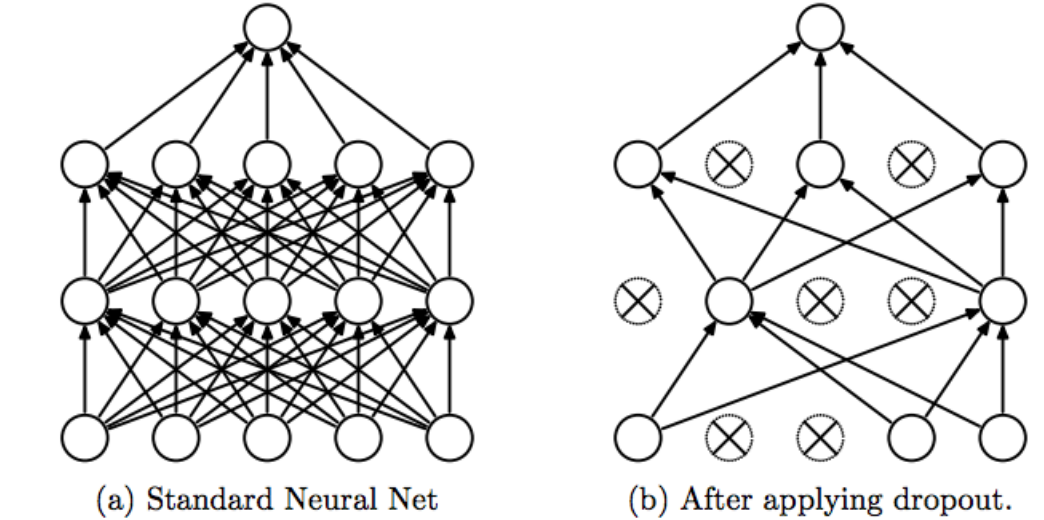
\includegraphics[scale=0.4]{chap3/image/dropout.png}
    \end{center}
    \caption{Dropout với p =0.5 và (b) là một subsample}
    \label{fig:dropout}
    \end{figure}
\end{center}

Cách hoạt động của dropout
\begin{itemize}
\item[•] Dropout được áp dụng trên một layer của mạng neural networks với một xác suất $\textbf{p}$ cho trước (có thể sử dụng nhiều Drop-Out khác nhau cho những layer khác nhau, nhưng trên 1 layer sẽ chỉ có 1 dropout)
\item[•] Tại mỗi step trong quá trình training, khi thực hiện feedforward đến layer sử dụng dropout, thay vì tính toán tất cả unit có trên layer, tại mỗi unit ta "gieo xúc xắc" với xắc suất $p$ xem unit đó được tính (active) hay không được tính (deactive). Những unit active ta tính toán bình thường còn với những unit deactive thì ta set giá trị tại unit đó bằng 0
\item[•] Trong quá trình test thì tất cả các unit đều được active và chúng ta mong muốn đầu ra của các units giống với đầu ra mong đợi trong quá trình trainning. Ví dụ đầu ra của một unit (trước khi drôput) là $\textbf{a}$, khi áp dụng dropout thì đầu ra mong đợi của unit đó sẽ là $\textbf{p}\textbf{a} + (1-\textbf{p})0$, vì unit bị deactive thì giá trị của unit đó là 0. Do đó trong quá trình test chúng ta điều chỉnh đầu ra $\textbf{a} \to \textbf{p}\textbf{a}$ để  giống với đầu ra mong đợi.
\end{itemize} \par
Thời gian test khá là quan trọng nên nếu chúng ta điều chỉnh đầu ra ở các layer áp dụng dropout thì hiệu suất test sẽ bị giảm đi. Vì thế thay vì chỉnh trong quá trình test thì chúng ta sẽ thực hiện việc này trong quá trình trainning. Ta sẽ lấy \textit{dropout mask} (vector xắc suất được khởi tạo ngẫu nhiên, tại vị trí có giá trị nhỏ hơn $p$ sẽ được giữ nguyên còn lớn hơn $p$ sẽ set lại giá trị vị trí đó là 0) chia cho $p$ trong quá trình trainning. Trường hợp này được gọi là \textit{inverted dropout}.
\end{enumerate}

\chapter{Convolutional Nerual Networks}
\label{chap:chap4}

\section{Tổng quan}
\textit{Convolutional Neural Network }(CNNs – Mạng nơ-ron tích chập) là một trong những mô hình Deep Learning tiên tiến giúp cho chúng ta xây dựng được những hệ thống thông minh với độ chính xác cao. Trong khóa luận này, tôi sẽ trình bày về  Convolution (tích chập) cũng như xây dựng mô hình CNNs cho bài toán nhận dạng chữ viết tay trong tiếng Nhật (Image Classification).\par
Lấy cảm hứng từ xử lý ảnh nên đầu vào và các lớp của CNNs có dạng như một bức ảnh chứ không có dạng vector như Neural Networks thông thường. Cụ thể, một bức ảnh sau khi số hoá có dạng \textit{width $\times$ height $\times$ depth} (width: số lượng điểm ảnh trên chiều rộng, height: số lượng điểm ảnh trên chiều cao, depth: số lượng kênh chẳng hạn như RGB có 3 kênh đại diện cho mức độ của 3 màu Đỏ, Lục, Lam). Mô hình được mô tả ở Hình \ref{fig:conv}

\begin{center}
\begin{figure}[H]
\label{fig:conv}
\begin{center}
\subfloat[mạng nơron thông thường]
  {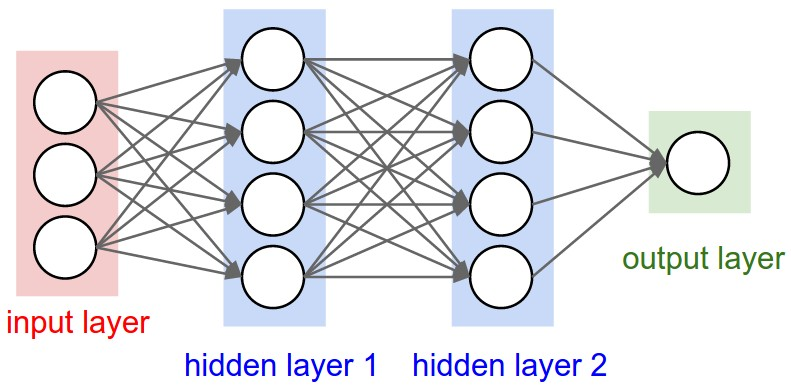
\includegraphics[width=.3\linewidth]{chap4/image/architectureNNs}}
\subfloat[mạng nơron tích chập]
  {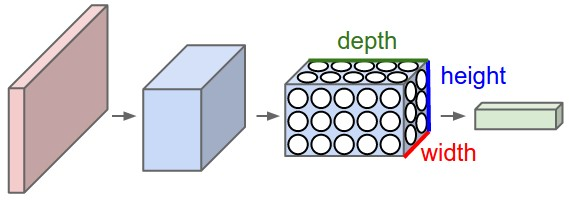
\includegraphics[width=.3\linewidth]{chap4/image/architectureCNN}}
\caption{Kiến trúc hai mạng}
\end{center}

\end{figure}
\end{center}

Một mạng CNNs đơn giản có ba lớp chính: lớp tích chập (\textit{convolutional layer}), lớp giảm số chiều (\textit{pooling layer}), lớp fully-connected. Các lớp convolutional và lớp pooling được xếp xen kẽ nhau Hình \ref{fig:convNetArch}.
\begin{center}
\begin{figure}[H]
	\begin{center}
		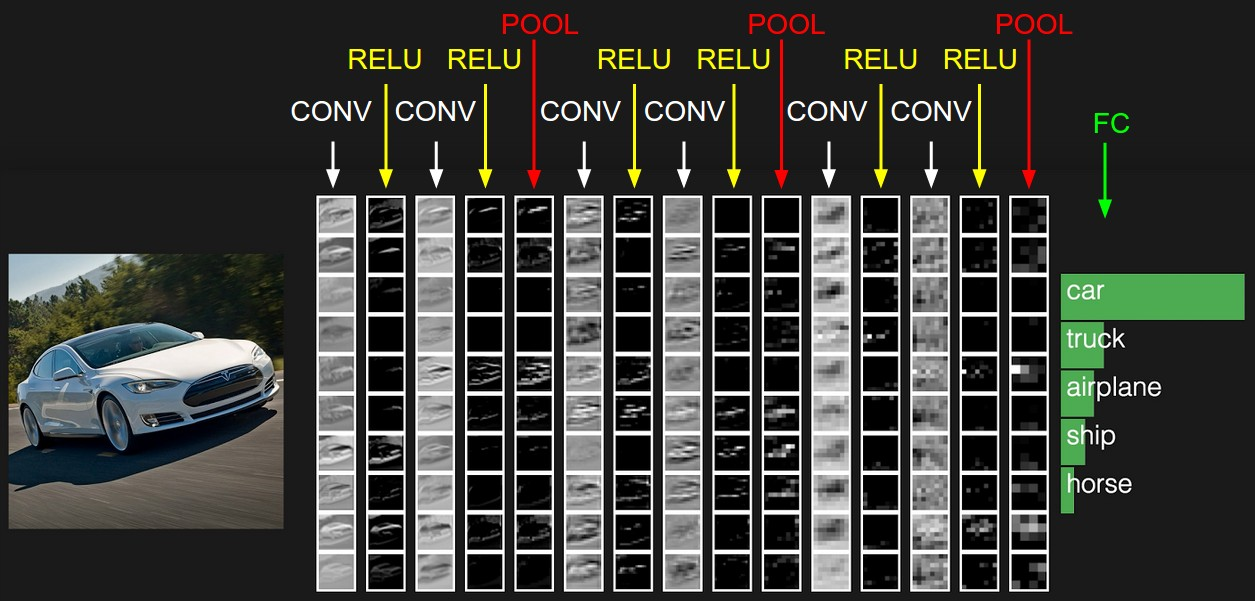
\includegraphics[scale=0.2]{chap4/image/convnet.jpeg}
	\end{center}
	\caption{ví dụ về kiến trúc của ConvNets}
	
\label{fig:convNetArch}
\end{figure}
\end{center}
\section{Bộ lọc và cửa sổ trượt}
Trước khi đi đến chi tiết các lớp, chúng ta cần hiểu \textit{bộ lọc (filter)} là gì, \textit{cửa sổ trượt (sliding window)} là gì.
\subsection{Bộ lọc - filter}
Như tôi đã trình bày ở phần trên, kích thước của đầu vào đã thay đổi thành dạng khối. Vì thế kích thước của trọng số cũng được thay đổi thành dạng khối để phù hợp với hình dạng của đầu vào và nó còn được gọi là \textit{filter} hoặc \textit{kennel}.  Ví dụ như Hình \ref{fig:filter}, ma trận I là ma trận đầu vào, ma trận K là filter và ma trận I*K là ma trận kết quả (được trình bày ở phần sau).
\begin{center}
\begin{figure}[htp]
	\begin{center}
		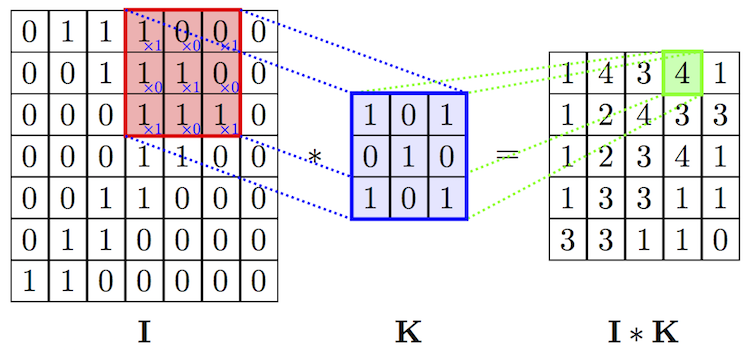
\includegraphics[scale=1.2]{chap4/image/minhHoaTichChap.png}
	\end{center}
	\caption{Bộ lọc - filter}
	\label{fig:filter}
\end{figure}
\end{center}
Kích thước của các filter thường là $d\times3\times3$, $d\times5\times5$, $d\times7\times7$  hoặc $d\times11\times11$, trong đó $d$ là chiều sâu của filter, hai tham số tiếp theo thể hiện chiều rộng và chiều cao của filter. Chú ý rằng chiều sâu của filter luôn luôn bằng chiều sâu của đầu vào.
\subsection{Cửa sổ trượt - sliding window}
\textit{Cửa sổ trượt (sliding window)} là ta chọn một "cửa sổ" có kích thước nhỏ hơn kích thước đầu vào và trượt cửa sổ đó trên đầu vào theo chiều ngang và chiều dọc. Các bước trượt là khoảng cách mà ta dịch chuyển filter trên đầu vào và đó gọi là \textit{stride}, ký hiệu là $s$. Ví dụ như Hình \ref{fig:slidingwindow}, ta có đầu vào kích thước là $5\times5$, cửa sổ có kích thước là $3\times3$ và tại mỗi bước trượt cửa sổ dịch chuyển đi một đơn vị, do đó stride bằng 1.
\begin{center}
\begin{figure}[htp]
	\begin{center}
		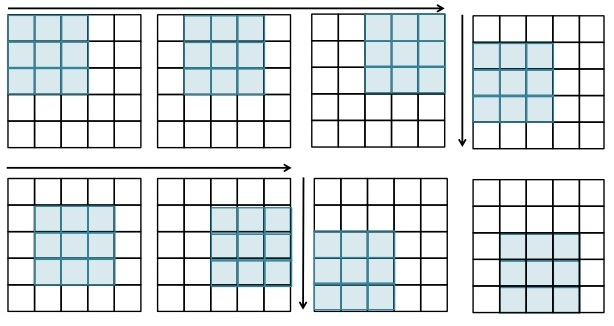
\includegraphics[scale=1]{chap4/image/slidingwindow.jpg}
	\end{center}
	\caption{Sliding window}
	\label{fig:slidingwindow}
\end{figure}
\end{center}

\section{Lớp tích chập - Convolutional layer}
Convolution layer là khối cốt lõi, cơ bản của ConvNets, lớp này chủ yếu nặng về việc tính toán. Lớp này chính là nơi thể hiện tư tưởng ban đầu của mạng nơron tích chập. Thay vì kết nối toàn bộ điểm ảnh, lớp này sẽ sử dụng bộ lọc (\textit{filter}) áp vào một vùng trong ảnh và tiến hành tính tích chập giữa bộ filter và giá trị điểm ảnh trong vùng cục bộ đó,  vùng này ta gọi là \textit{receptive filter}. Sau đó ta dùng sliding window để trượt filter và tiến hành tích chập tại mỗi vùng ta trượt đến. Tôi sẽ trình bày chi tiết thông qua Hình  \ref{fig:tinhtoanConv}.

\begin{figure}[htp]

\subfloat[\label{fig:slide1_1}]
  {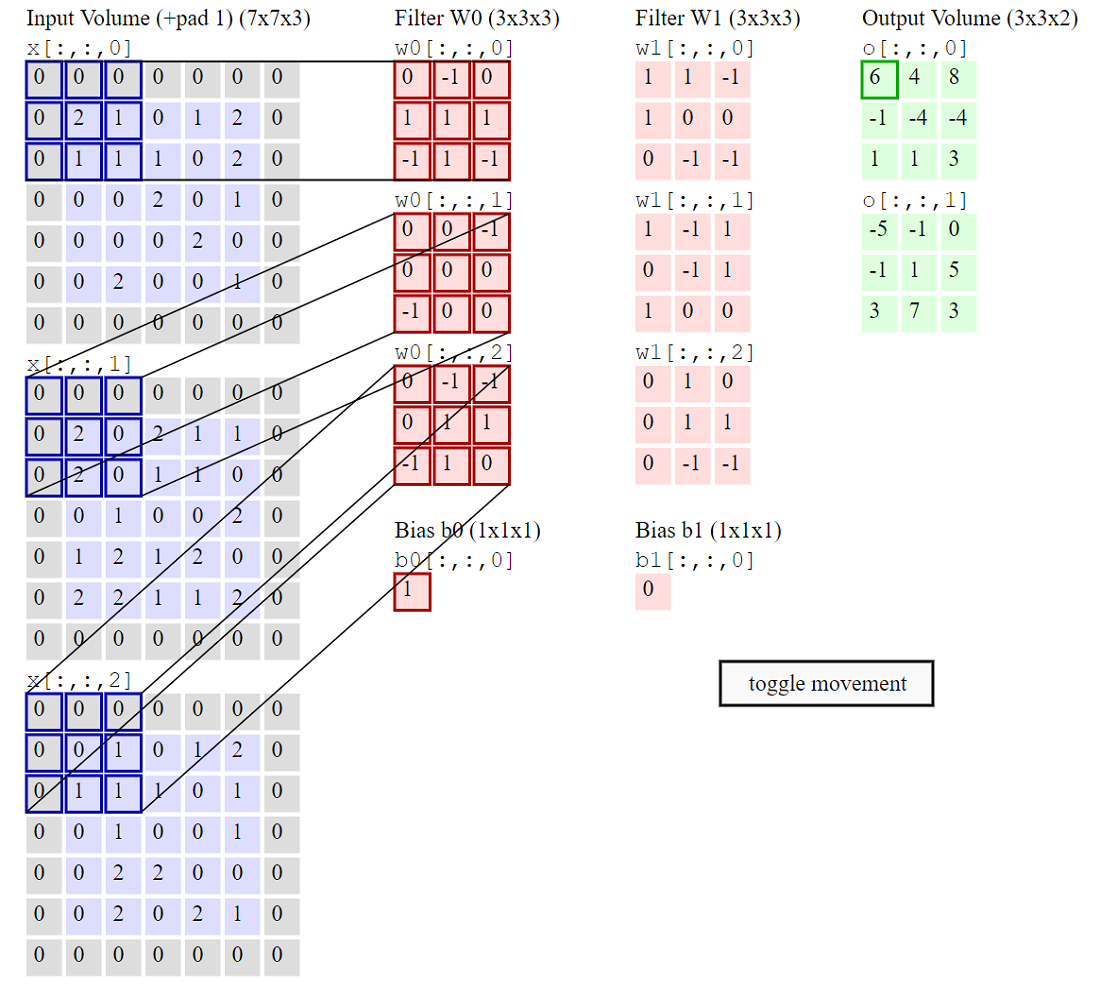
\includegraphics[width=.3\linewidth]{chap4/image/slide1_1.png}}\hfill
\subfloat[\label{fig:slide1_2}]
  {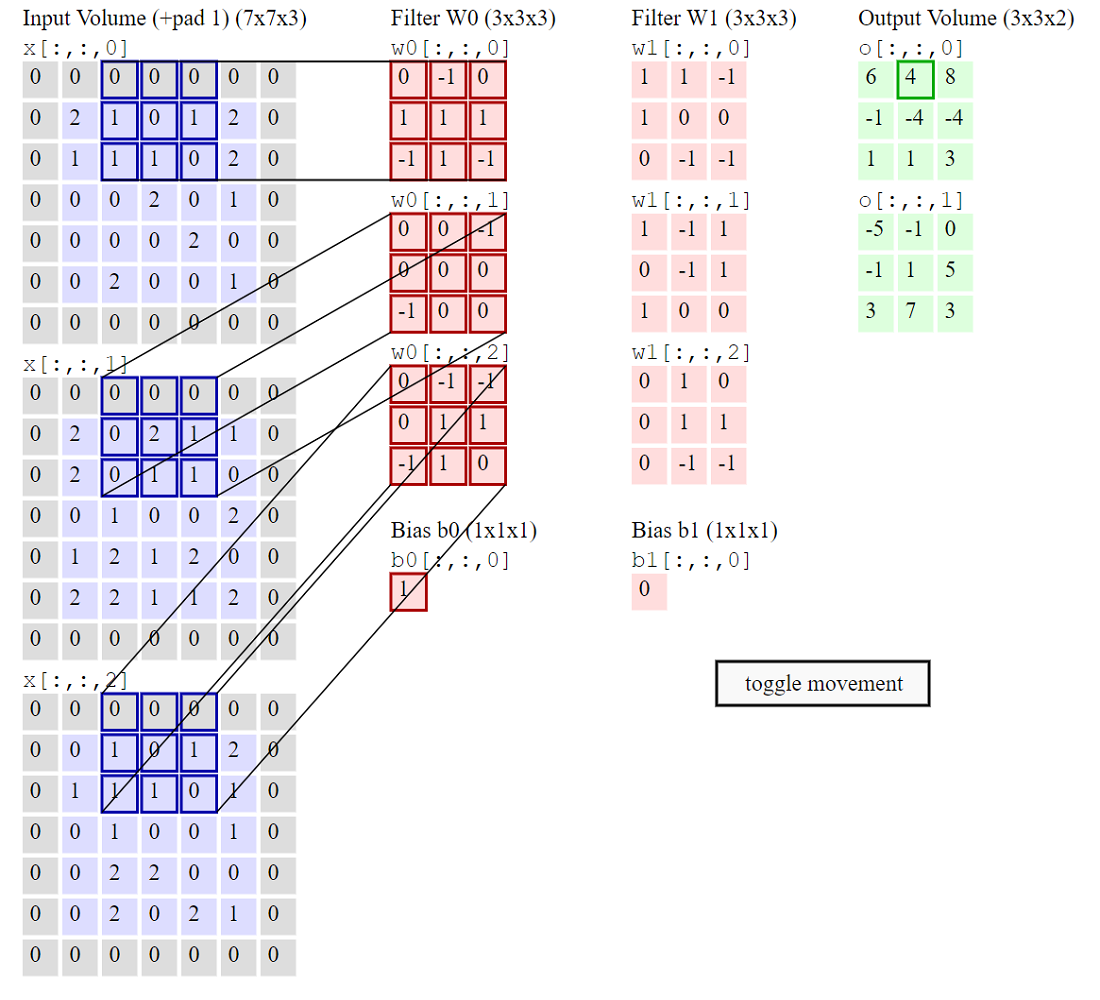
\includegraphics[width=.3\linewidth]{chap4/image/slide1_2.png}}\hfill
\subfloat[\label{fig:slide1_3}]
  {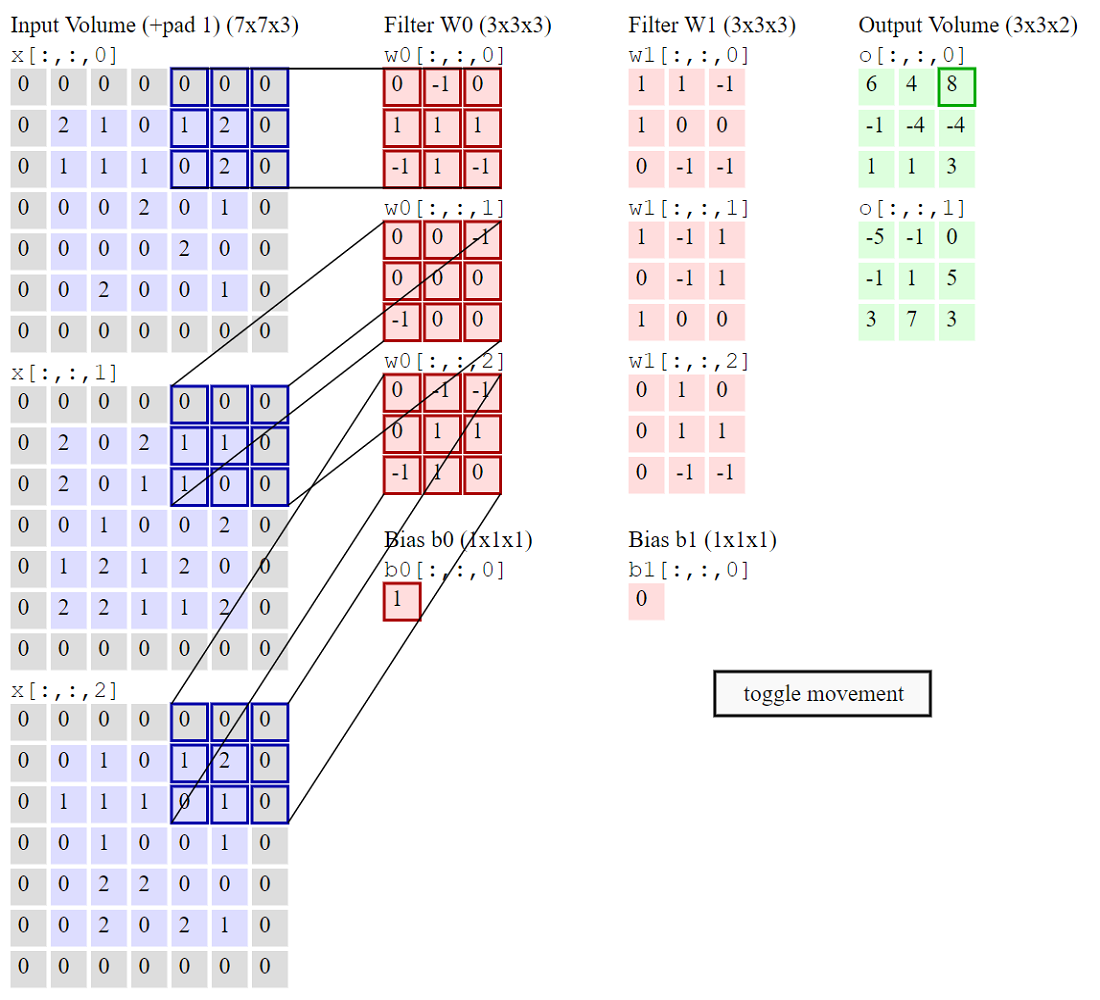
\includegraphics[width=.3\linewidth]{chap4/image/slide1_3.png}}\\
\subfloat[\label{fig:slide2_1}]
  {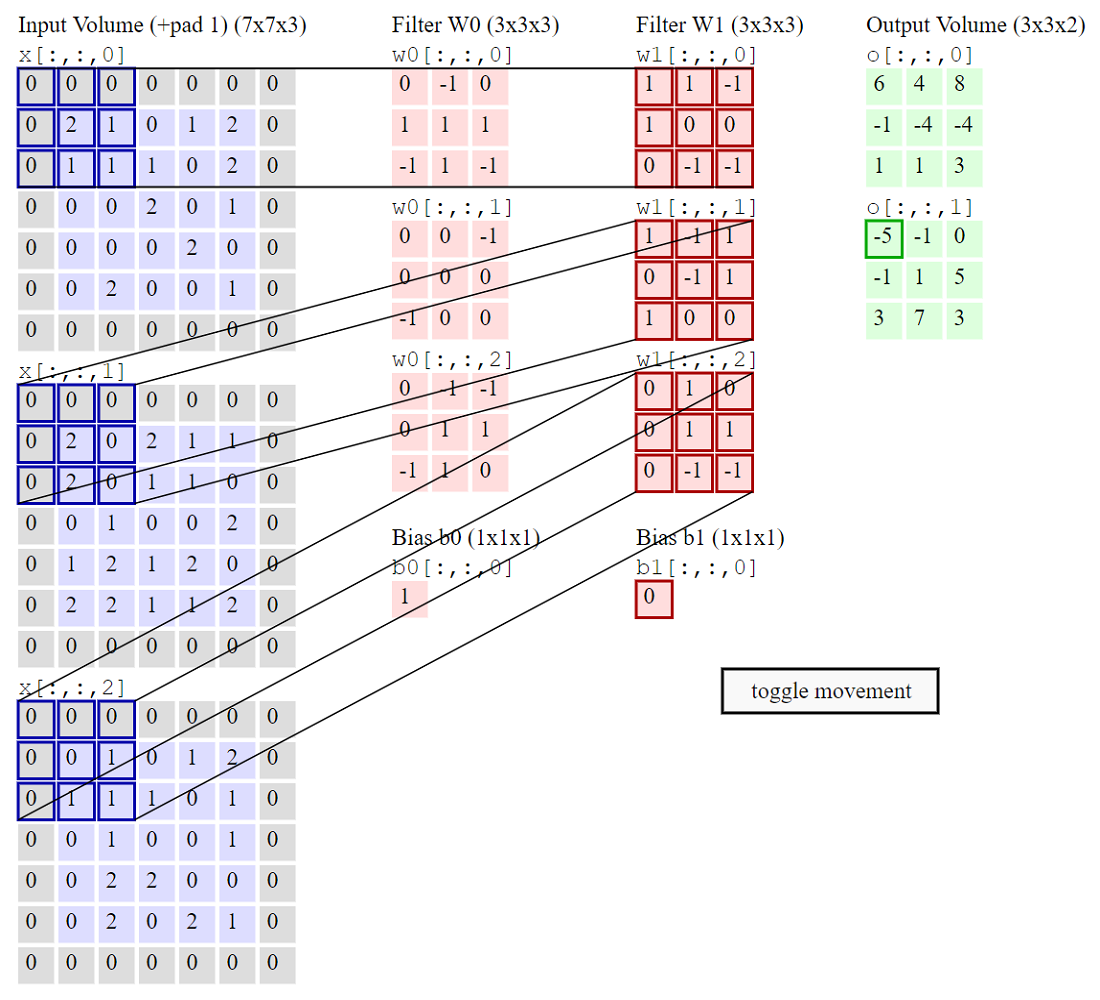
\includegraphics[width=.3\linewidth]{chap4/image/slide2_1.png}}\hfill
\subfloat[\label{fig:slide2_2}]
  {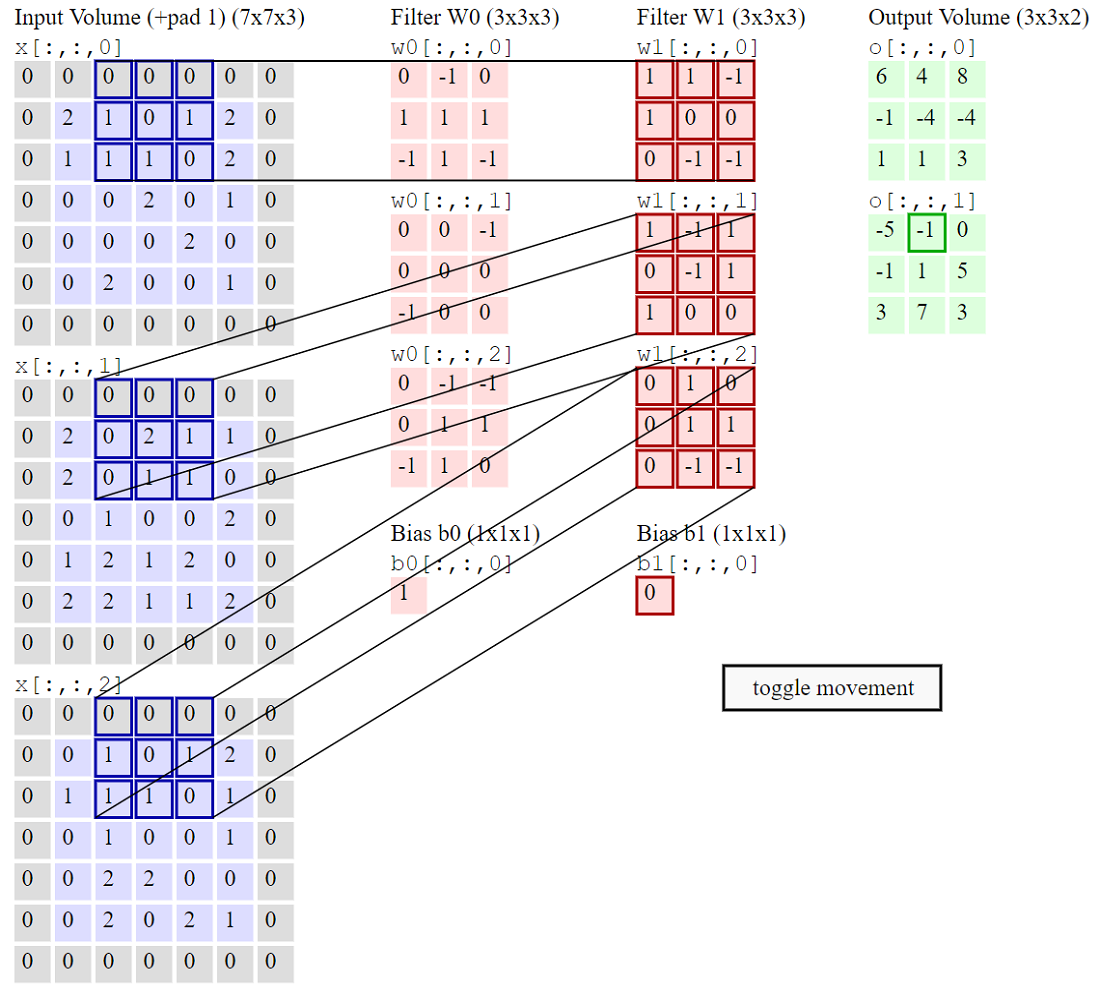
\includegraphics[width=.3\linewidth]{chap4/image/slide2_2.png}}\hfill
\subfloat[\label{fig:slide2_3}]
  {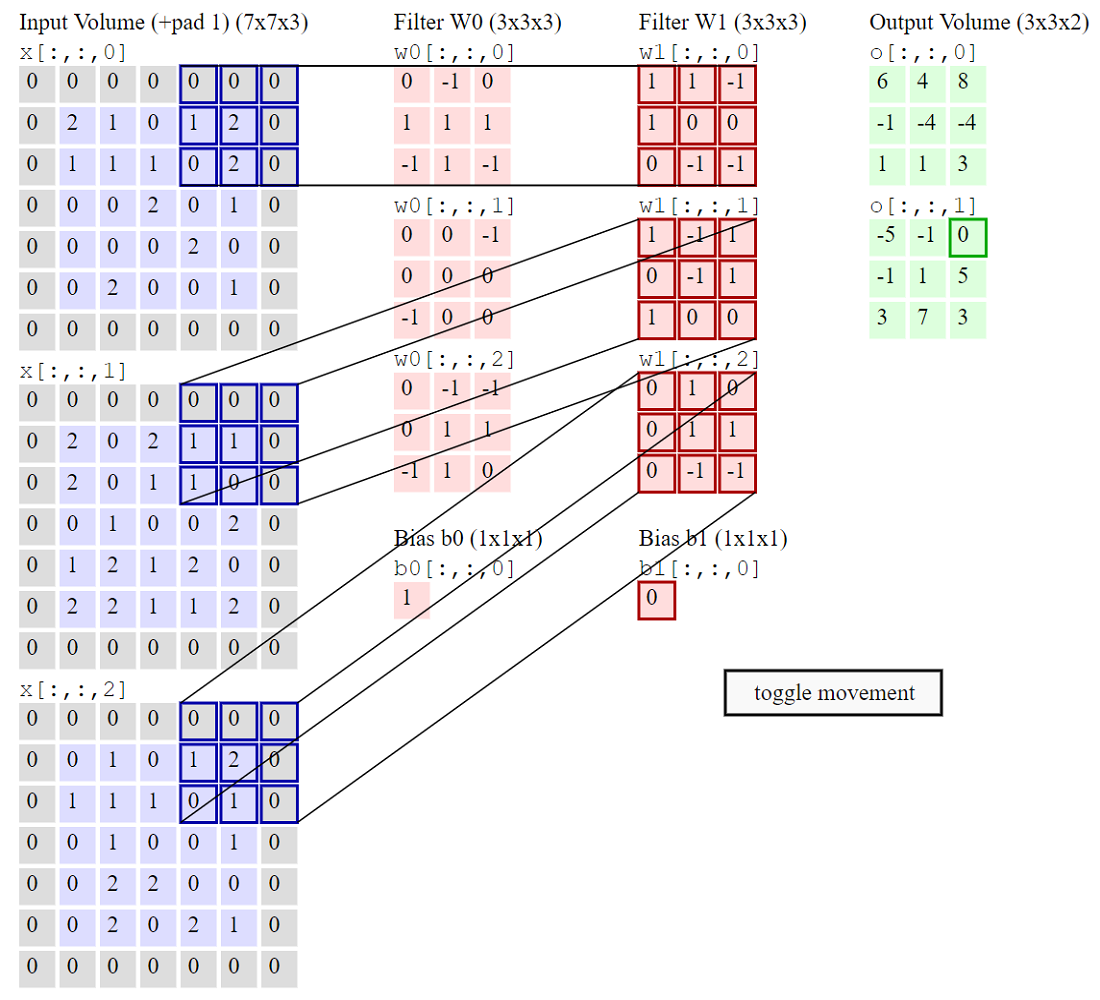
\includegraphics[width=.3\linewidth]{chap4/image/slide2_3.png}}
\caption{Tính toán trong lớp tích chập}
\label{fig:tinhtoanConv}
\end{figure}

Theo Hình \ref{fig:tinhtoanConv} ta có kích thước đầu vào là $7 \times 7\times 3$, stride bằng 2, kích thước filter là  $2\times 3\times 3 \times 3$ với 2 là số \textit{channel} (số chanel sẽ là chiều sâu output chúng ta mong muốn). Tại Hình \ref{fig:slide1_1} ta  thực hiện phép tính... tương ứng giữa receptive filter, $filter ~W0$ tại tất cả các độ sâu, kết quả được cộng thêm $bias$ rồi lưu vào ma trận output vị trí đầu tiên của đầu ra. Sau đó ta thực hiện cách tính toán trên kết hợp sliding window với stride bằng 2 và filter là $filter W0$, kết quả ta thu được là ma trận output thứ nhất, các Hình \ref{fig:slide1_1}, \ref{fig:slide1_2}, \ref{fig:slide1_3} mô tả giai đoạn này. Và tương tự như trên ta thực hiện với $filter ~W1$ theo Hình \ref{fig:slide2_1}, \ref{fig:slide2_2}, \ref{fig:slide2_3} ta thu được kết quả là ma trận thứ hai tại output. Như vậy nếu ta có càng nhiều channel thì chiều sâu output của chúng ta càng lớn. \par

Nếu như đầu ta chỉ tính trên kích thước đầu vào thì với filter $3\times 3$ và stride bằng 2 thì ta chỉ trượt được hai lần và đến hàng, cột thứ 5 của đầu vào còn giá trị tại hàng, cột thứ 6, 7 sẽ không được tính. Vì thế chúng ta thêm vào ma trận đầu vào các hàng và cột đối xứng với giá trị bằng 0 để không ảnh hưởng đến đầu vào mà khi đó ta sẽ quét được hết các giá trị của đầu vào. Cách này được gọi là \textit{zero padding}. Như ở ví dụ trên ta thấy đầu vào được bao quanh bởi các số 0 và kích thước tăng thành $8 \times 8$, đó là ta áp dụng zero padding với p=1.\par
Ta có công thức để tính toán kích thước đầu ra như sau:
\begin{itemize}
	\item Kích thước đầu vào \textbf{$W_1$} x \textbf{$H_1$} x \textbf{$D_1$} (rộng x cao x sâu)
	\item Kích thước của filter \textbf{$F$}
	\item Số channel \textbf{$K$}
	\item Tốc độ trượt \textbf{$S$}
	\item Giá trị của zero-padding \textbf{$P$}
	\item Kích thước đầu ra \textbf{$W_2$} x \textbf{$H_2$} x \textbf{$D_2$}:
	\begin{itemize}
		\item[+]  \textbf{$W_2 = (W_1 - F+ 2P)/S +1$}
		\item[+] \textbf{$H_2 = (H_1 - F+ 2P)/S +1$}
		\item[+] \textbf{$D_2 = K$}
	\end{itemize}	 
\end{itemize}	

\begin{center}
\begin{figure}[htp]
	\begin{center}
		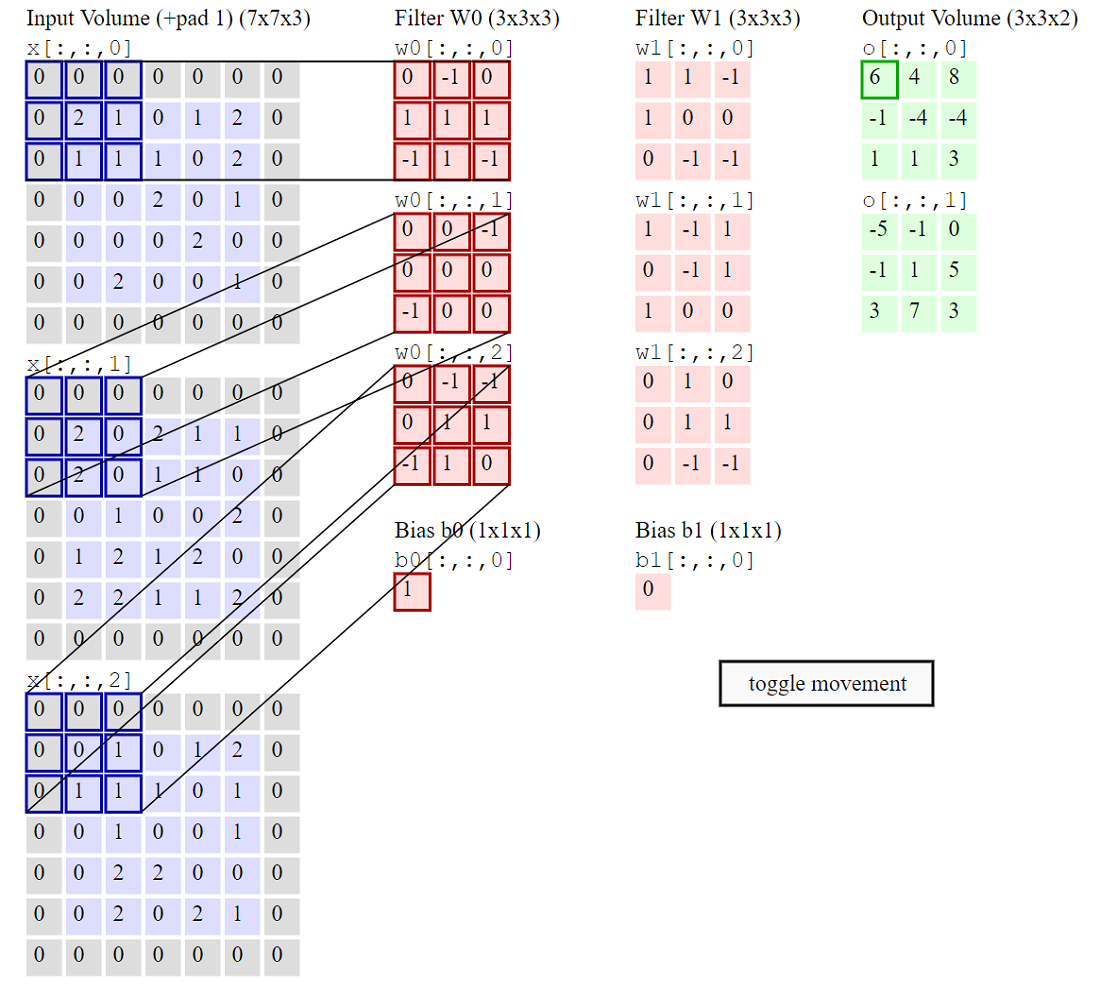
\includegraphics[scale=0.2]{chap4/image/slide1_1.png}
	\end{center}
	\caption{Ví dụ về tính toán kích thước đầu ra}
	\label{fig:minhhoatichchap2}
\end{figure}
\end{center}
Giả sử ta có thông số như hình \ref{fig:minhhoatichchap2} với kích thước đầo vào là $7\times7\times3$ tương đương $W=H=7,~ D_1=3$;stride $S=3$; kích thước filter là $2\times 3\times 3 \times 3$ hay $F=3$ và số channel $K=2$. Theo công thức ta tính được $(W_1 - F+ 2P)/S$ không phải là số nguyên do đó ta cần thêm padding để giá trị này là số nguyên. Ta chọn $P=1$ vì $(7-3+2\times 1)/3 +1$ là số nguyên. Như vậy ta tính được kích thước đầu ra sẽ là $3\times3\times2$. \par
Một phần quan trọng của layer này đó là hàm activation, hàm này được tính với đầu vào là kết quả sau khi thực hiện tích chập. Và ReLU thường được chọn là hàm activation do tính đơn giản của nó. Nhiệm vụ của nó là chuyển toàn bộ giá trị âm trong kết quả sau khi tích chập thành 0. Ý nghĩa của cách cài đặt này chính là tạo nên tính phi tuyến cho mô hình. 
\section{Lớp giảm số chiều -  pooling layer}
\textit{Lớp giảm số chiều (pooling layer)} trong mạng CNNs thực hiện công việc loại bỏ bớt những thông tin không cần thiết sau khi thực hiện tích chập và được chèn giữa các lớp convolutional với nhau hoặc sau một tập lớp convolutional. Nó có vai trò giảm kích thước dữ liệu. Với một bức ảnh kích thước lớn qua nhiều lớp pooling sẽ được thu nhỏ lại tuy nhiên vẫn giữ được những đặc trưng cần cho việc nhận dạng (thông qua cách lấy mẫu). Việc giảm kích thước dữ liệu sẽ làm giảm lượng tham số, tăng hiệu quả tính toán và góp phần kiểm soát hiện tượng quá khớp (overfitting). Tuy nhiên nếu lạm dụng loại layer này cũng có thể khiến data đi qua bị mất dữ liệu.\par
\textbf{Cách thức hoạt động}: Pooling layer sử dụng sliding window và tại mỗi cửa sổ trượt trên đầu vào chỉ có một giá trị được xem là giá trị đại diện cho thông tin ảnh tại vùng đó (giá trị mẫu) được giữ lại và đó gọi là tiến hành lấy mẫu (\textit{subsampling}). Các phương thức lấy phổ biến trong pooling layer là \textit{Max pooling} (lấy giá trị lớn nhất), \textit{Min pooling} (lấy giá trị nhỏ nhất) và \textit{Average Pooling} (lấy giá trị trung bình). Hình \ref{fig:pool} mô tả tiến hành lấy mẫu bằng max pooling.\par

\begin{center}
\begin{figure}[H]
	\begin{center}
		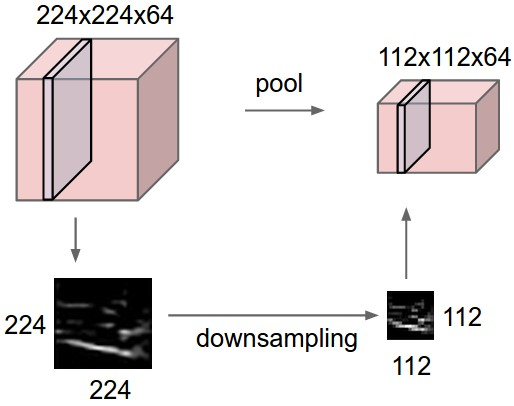
\includegraphics[scale=0.5]{chap4/image/poolEx.jpeg}
	\end{center}
	\caption{Minh họa giảm số chiều}
	\label{fig:pool}
\end{figure}
\end{center}

Ví dụ ta có ma trận đầu vào $4\times 4$  như hình \ref{fig:poolExample}, với kích thước cửa sổ áp dụng cho slidiing window là $2\times 2$ và stride = 2, điều này tương đương với việc ta chia ma trận đầu vào thành 4 ma trận con với kích thước là $2\times2$.  Phương thức ta áp dụng tại đây là max pooling, do đó tại mỗi cửa sổ khi ta áp vào đầu vào thì ta sẽ chọn giá trị lớn nhất làm đại diện cho cửa sổ đó và ta thu được kết quả là ma trận $2\times2$ bên tay phải.\par
\begin{center}
\begin{figure}[htp]
	\begin{center}
		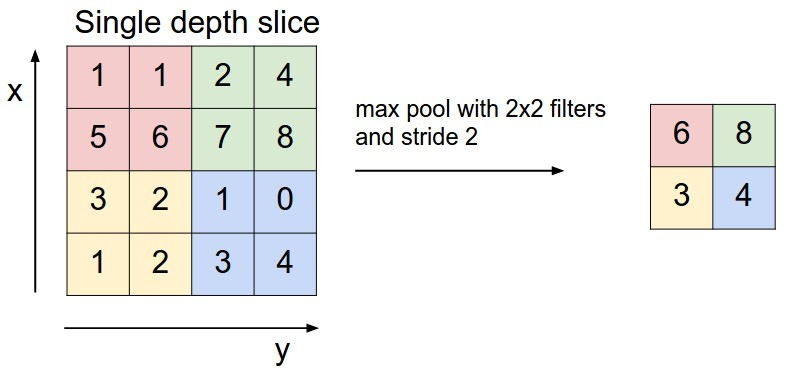
\includegraphics[scale=0.5]{chap4/image/maxpoolEx.jpeg}
	\end{center}
	\caption{Max pooling}
	\label{fig:poolExample}
\end{figure}
\end{center}
Ta rút ra được công thức tính kích thước đầu ra cho lớp này như sau:
\begin{itemize}
	\item Kích thước đầu vào \textbf{$W_1$} x \textbf{$H_1$} x \textbf{$D_1$} (rộng x cao x sâu),
	\item Kích thước cửa sổ \textbf{$F$},	
	\item Tốc độ trượt \textbf{$S$}
	\item Kích thước đầu ra \textbf{$W_2$} x \textbf{$H_2$} x \textbf{$D_2$}:
	\begin{itemize}
		\item  \textbf{$W_2 = (W_1 - F)/S +1$}
		\item  \textbf{$H_2 = (H_1 - F)/S +1$}
		\item \textbf{$D_2 = D_1$}
	\end{itemize}	 
\end{itemize}
Chú ý rằng chúng ta không thường xuyên sử dụng $zero~padding$ cho lớp này.
\section{Lớp Fully-Connected (Fully-Connected layer)}
Sau khi ảnh được xử lý và trích xuất đặc trưng bằng các lớp convolutional, pooling thì ta sẽ làm phẳng (flatten) output cuối cùng của giai đoạn trước đó và áp dụng mạng nơron truyền thẳng với input là dữ liệu ta vừa làm phẳng. Hay nói cách khác Fully-Connected chính là một mạng nơron được gắn vào phần cuối của CNNs với input là đầu ra của các lớp trước đó. Nó đóng vai trò như một mô hình phân lớp và tiến hành dựa trên dữ liệu đã được xử lý ở các lớp trước đó.
\section{Tổng kết}
Dưới đây là một mô hình mạng CNNs kết hợp giữa các layer với nhau với cấu trúc như sau: Conv $\to$ Max-pool $\to$ Conv (giữ nguyên kích thước) $\to$ Max-pool $\to$ Conv (giữ nguyên kích thước) $\to$ Conv (giữ nguyên kích thước) $\to$ Conv (giữ nguyên kích thước) $\to$ Max-pool $\to$ Flatten $\to$ FC . Kích thước các lớp được thể hiện tại Hình \ref{fig:CNN}.
\begin{center}
\begin{figure}[H]
	\begin{center}
		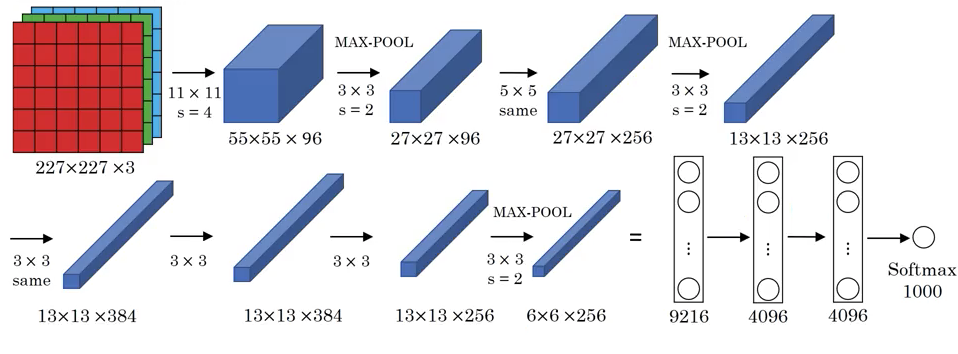
\includegraphics[scale=0.5]{chap4/image/CNN.png}
	\end{center}
	\caption{Ví dụ cấu trúc mạng CNNs}
	\label{fig:CNN}
\end{figure}
\end{center}


\section{câu hỏi}
\begin{enumerate}
\item làm nào để thụt lề đoạn đầu của mỗi phần section, subsection
\item căn chỉnh công thức căn lề trái (hiện đang bị căn giữa) phần feedforward
\item Công thức backpropagation: đạo hàm 2 cái khác nhau
\end{enumerate}

\end{document}